\documentclass{article} % For LaTeX2e
\usepackage{iclr2027_conference,times}
\input{math_commands.tex}

\usepackage{booktabs}
\usepackage{amsmath,amssymb}
\usepackage{graphicx}
\usepackage{caption}
\usepackage{multirow}
\usepackage{array}
\usepackage{pifont}
\usepackage{hyperref}
\usepackage{url}
\setlength{\tabcolsep}{4pt}

% ---- Title ----
\title{Discover, Attribute, Explain: A Minimal Framework for Evidence-Grounded Microbiome Diagnosis}
\author{Jinxu Liu}
\date{}

\begin{document}
\maketitle

\begin{abstract}We present SimpleEmb, a microbiome framework decoupling disease classification from biological interpretation. On clean\_2538 IBD (659 train, 167 test), a minimal encoder (nn.Embedding + masked mean pooling, no pretraining, no Transformer) achieves 92.57\% accuracy (AUC 0.975), comparable to tree ensembles (XGBoost 92.22\%; HistGradientBoosting 92.5\% grouped-CV) and 41.7pp above a 34M pretrained MGM Transformer. Embedding dimension saturates at $E{=}512$. LOO attribution is reliable (Spearman $\rho{=}0.72$), and LOO-grounded Qwen2-7B explanations halve hallucination (0.72 to 0.36) with 98\% consistency and 0.94 direction accuracy. Leave-one-source-out validation across five cohorts confirms batch effects remain the central challenge. SimpleEmb shows the model discovers patterns, LOO provides evidence, and the LLM explains the evidence.\end{abstract}

% ═══════════════════════════════════════
% 1. INTRODUCTION
% ═══════════════════════════════════════
\section{Introduction}

Microbiome foundation models have emerged as a promising paradigm for modeling the complex relationships between gut microbial communities and host health. Recent models including MGM~\citep{mgm2024}, Waypoint~\citep{waypoint2026}, and ProCyon~\citep{procyon2025} follow a common blueprint: tokenize genus abundance profiles, encode them with a Transformer, and fine-tune on downstream tasks.

However, three critical questions remain under-explored:

\begin{enumerate}
  \item \textbf{Architecture necessity}: Do genus-level microbiome classification tasks actually benefit from Transformer encoders and large-scale pretraining?
  \item \textbf{LLM role}: Should large language models serve as classifiers, or as reasoning interfaces on top of a specialized classifier?
  \item \textbf{Evidence grounding}: Can model explanations be verified against literature and made robust across data splits?
\end{enumerate}

This paper systematically investigates these questions through controlled experiments. Our findings challenge several assumptions in current microbiome foundation model design and lead to SimpleEmb: a simple embedding-based classifier with LOO-attributed feature importance, where the LLM serves solely as an interpreter --- not a predictor.

\textbf{Contributions:}
\begin{itemize}
  \item \textbf{Architecture minimalism}: SimpleEmb (nn.Embedding + mean pool + MLP, 1.1M params, random init) achieves 92.57\% ACC, exceeding MGM's 34M-param pretrained Transformer (50.9\%) by 41.7pp
  \item \textbf{Comprehensive baseline comparison}: 9 methods compared on identical train/test split with 6 performance metrics
  \item \textbf{Component ablation}: Isolate contributions of embedding, random projection, non-linearity, and end-to-end training
  \item \textbf{Embedding dimension analysis}: Performance saturates at $E{=}512$ (91.4\% grouped-CV, 93.4\% held-out; 760K params)
  \item \textbf{Cross-dataset transfer}: Training on $5\times$ larger diverse data improves cross-dataset generalization by 26.8pp
  \item \textbf{LOO Attribution Reliability}: Spearman $\rho{=}0.72$ rank consistency, deletion test validation, literature direction agreement (5/6)
  \item \textbf{LLM explanation benchmark} ($n{=}167$): LOO grounding halves hallucination (0.72 to 0.36/response), achieves 98\% consistency and 0.94 direction accuracy
\end{itemize}

% ═══════════════════════════════════════
% 2. RELATED WORK
% ═══════════════════════════════════════
\section{Related Work}

\textbf{MGM}~\citep{mgm2024} introduced the first large-scale microbiome foundation model: an 8-layer Transformer pretrained with autoregressive next-genus prediction on MicroCorpus-260K (263,302 samples, 9,665 genera). MGM demonstrated cross-regional diagnosis, keystone genus discovery via attention analysis, and in silico perturbation experiments. Its rank-based encoding mitigates extreme abundance values but discards relative abundance information.

\textbf{BiomeGPT}~\citep{biomegpt2026} is a transformer-based foundation model pretrained on 13,300 species-level human gut metagenomes spanning 32 phenotypes. It uses a dual embedding strategy (species embedding + quantile-based abundance bin embedding) with masked abundance prediction. Its CLS-token attention analysis revealed that attention is not driven by prevalence alone, and correlations with differential abundance were task-dependent ($\rho$ from $-0.05$ to $0.46$). Notably, BiomeGPT's model weights are not publicly available, preventing direct benchmarking.

\textbf{Waypoint/Atlas}~\citep{waypoint2026} scaled the Transformer approach to 539k+ samples with 6M--170M parameter variants.

\textbf{ProCyon}~\citep{procyon2025} coupled a protein encoder with an LLM for multimodal biomedical tasks, inspiring our dual-branch design --- though we ultimately adopted a fundamentally different encoder.



% ═══════════════════════════════════════
% 3. DATASET ANALYSIS
% ═══════════════════════════════════════
\section{Dataset Analysis}

Understanding the structure of microbiome data is essential before designing model architectures. We characterize the clean\_2538 dataset, which combines American Gut Project (AGP) and Fecal Transplantation Program (FTP) cohorts from the Qiita platform.

\subsection{Cohort Statistics}



\subsection{Genus Abundance Distribution}

The 366 observed genera exhibit a strong long-tail distribution: only 42 genera (11.5\%) appear in more than 50\% of samples, while 251 genera (68.6\%) are rare ($<$5\% prevalence). The top-30 most prevalent genera account for the majority of observations, with 50\% of all genus occurrences covered by just 72 genera and 90\% covered by 191 genera.

\begin{figure}[ht]
\centering
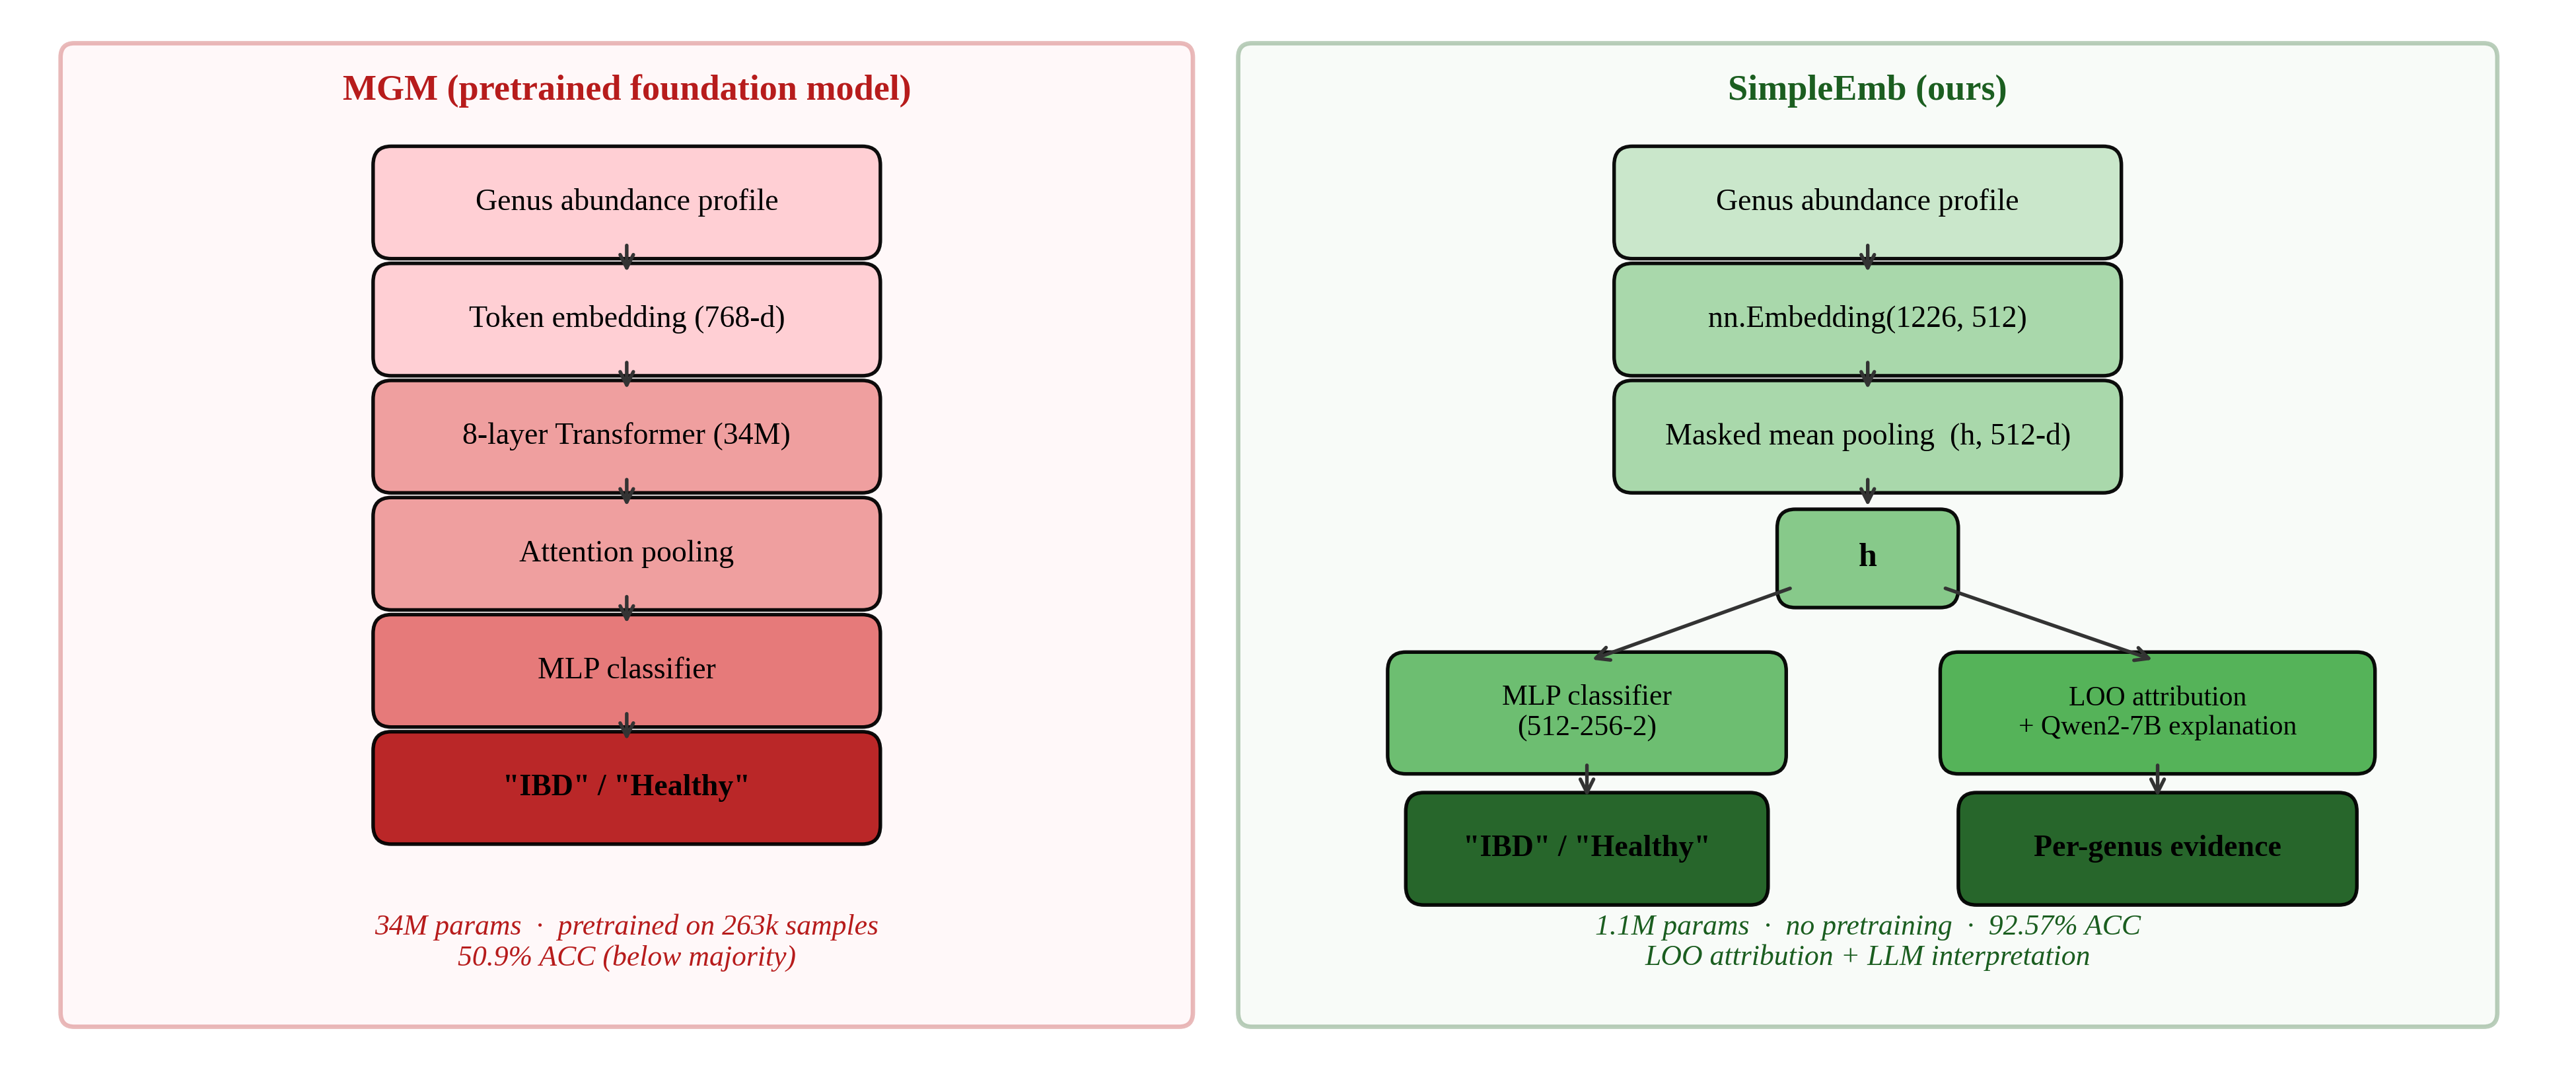
\includegraphics[width=0.62\textwidth]{figures/dataset_architecture_figure.png}
\caption{\textbf{Dataset statistics and architecture comparison.}
(A) SimpleEmb vs.\ MGM architecture side-by-side. (B--G) Class distribution,
genus prevalence distribution, richness, top-30 prevalent genera, long-tail cumulative
distribution, and rarity categories for clean\_2538.}
\label{fig:dataset}
\end{figure}

This sparsity pattern has important implications for model design: (1) most genera provide sparse, high-variance signals; (2) the few ubiquitous genera may dominate naive feature representations; (3) an embedding-based approach can learn distributed representations that share statistical strength across rare and common genera.

\subsection{Disease Heterogeneity}

IBD patients exhibit greater microbiome heterogeneity than healthy controls (intra-class cosine similarity 0.54 vs. 0.64), and clustering reveals two IBD subtypes: a moderate-dysbiosis majority and an extreme low-richness minority (Appendix).

\section{Methods}

\subsection{SimpleEmb Architecture}

SimpleEmb adopts a minimalist design based on systematic ablation findings:

\begin{center}
\begin{tabular}{c}
\textbf{Input}: Genus abundance profile $[g_1, g_2, \ldots, g_k]$ ($V{=}1226$, sorted by abundance) \\
$\downarrow$ \\
\textbf{SimpleEmb}: $\text{nn.Embedding}(1226, 768, \text{padding\_idx}{=}0)$ \\
$\downarrow$ masked mean pool \\
Patient representation $\mathbf{h} \in \mathbb{R}^{768}$ \\
$\downarrow$ \\
$\swarrow \qquad \qquad \qquad \searrow$ \\
\textbf{Classification Head} \hspace{2cm} \textbf{Explanation Head} \\
MLP($768{\rightarrow}256{\rightarrow}\text{BN}{\rightarrow}\text{ReLU}{\rightarrow}\text{Drop}{\rightarrow}2$) \quad LOO Attribution (per-genus) \\
$\downarrow$ \hspace{3.5cm} $\downarrow$ \\
$P(\text{IBD} \mid \text{microbiome})$ \hspace{2.3cm} Important genera + direction \\
\hspace{4.3cm} $\downarrow$ \\
\hspace{3.3cm} Qwen2-7B-Instruct \\
\hspace{3.3cm} $\downarrow$ \\
\hspace{2.3cm} Biological explanation
\end{tabular}
\end{center}

\textbf{Key design decisions:}
\begin{enumerate}
  \item \textbf{No Transformer}: Genus sequences sorted by abundance have no meaningful sequential structure. Each genus carries largely independent diagnostic information.
  \item \textbf{No pretraining}: The embedding is randomly initialized and trained end-to-end. MGM's next-genus pretraining objective does not transfer to IBD classification (see \S\ref{sec:baseline}).
  \item \textbf{Mean pooling}: Masked mean pooling over valid genus positions preserves more information than attention pooling.
  \item \textbf{Dual-branch separation}: Classification and explanation are decoupled --- each optimized for its specific role.
\end{enumerate}

\textbf{Model complexity}: 1.14M parameters (Embedding: 0.93M, MLP: 0.21M). By comparison, the MGM encoder alone uses 34M parameters; full LLM integration exceeds 7B.

\subsection{Baseline Methods}

We compare against nine baselines spanning three categories, all evaluated on the identical train/test split (659/167):

\begin{itemize}
  \item \textbf{Lower bound}: Majority class classifier
  \item \textbf{Classical ML} (on raw 1226-dim abundance): Logistic Regression, Linear SVM, Random Forest (200 trees), XGBoost (200 trees), MLP (sklearn, 256$\rightarrow$128)
  \item \textbf{MGM-based}: MGM pretrained encoder (34M params, 6 Transformer layers, pretrained on 263k samples) + MLP
  \item \textbf{SimpleEmb}: SimpleEmb + MLP, 5-seed ensemble
\end{itemize}

\subsection{Ablation Design}

To isolate each component's contribution:
\begin{itemize}
  \item \textbf{A: Raw$\rightarrow$MLP} --- Raw abundance directly to MLP (no embedding)
  \item \textbf{B: RandomEmb$\rightarrow$MLP} --- Frozen random embedding + mean pool $\rightarrow$ MLP
  \item \textbf{C: SimpleEmb$\rightarrow$Linear} --- Trained embedding + Linear classifier (no MLP)
  \item \textbf{D: SimpleEmb$\rightarrow$MLP (SimpleEmb)} --- Full model, end-to-end trained
\end{itemize}

\subsection{Design Borrowings}

We incorporate ideas from the microbiome-modeling literature while remaining far smaller than the sources: strict in-fold preprocessing and leave-one-source-out evaluation (SIAMCAT~\citep{siamcat2021}), LOO attribution and rank encoding (MGM~\citep{mgm2024}), abundance-bin embeddings and masked-abundance pretraining (BiomeGPT~\citep{biomegpt2026}), and denoising pretraining (DeepMicro~\citep{deepmicro2020}). Each is a single-module addition to the SimpleEmb backbone.

\subsection{Training Details}

All models trained with: AdamW ($\text{lr}{=}10^{-3}$, $\text{weight\_decay}{=}10^{-4}$), CosineAnnealing ($T_{\max}{=}50$), batch\_size${=}32$, class-weighted loss (Disease weight${=}1.5$). SimpleEmb reports mean $\pm$ std across 5 random seeds (42, 123, 456, 789, 1024).

% ═══════════════════════════════════════
% 4. EXPERIMENTS
% ═══════════════════════════════════════
\section{Experiments}

\subsection{Baseline Comparison}
\label{sec:baseline}

\begin{table}[ht]
\centering
\caption{\textbf{IBD classification performance on clean\_2538 (659 train / 167 test).}
All methods evaluated on identical split. Bold indicates best. SimpleEmb reports 5-seed ensemble mean $\pm$ std.}
\label{tab:baselines}
\begin{tabular}{lcccccc}
\toprule
\textbf{Method} & \textbf{ACC} & \textbf{AUC} & \textbf{Prec.} & \textbf{Rec.} & \textbf{F1} & \textbf{Params} \\
\midrule
\multicolumn{7}{l}{\textit{Lower bound}} \\
\;\; Majority class & 0.5569 & 0.5000 & 0.5569 & 1.0000 & 0.7154 & 0 \\
\midrule
\multicolumn{7}{l}{\textit{Classical ML (raw 1226-dim abundance)}} \\
\;\; Logistic Regression & 0.8802 & 0.9241 & 0.9195 & 0.8602 & 0.8889 & 2.5K \\
\;\; Linear SVM & 0.8563 & 0.8641 & 0.9367 & 0.7957 & 0.8605 & 2.5K \\
\;\; Random Forest & 0.8922 & 0.9587 & 0.9213 & 0.8817 & 0.9011 & $\sim$200 trees \\
\;\; XGBoost & 0.9222 & 0.9679 & 0.9348 & 0.9247 & 0.9297 & $\sim$200 trees \\
\;\; MLP (sklearn) & 0.8982 & 0.9605 & 0.9318 & 0.8817 & 0.9061 & 330K \\
\midrule
\multicolumn{7}{l}{\textit{MGM Transformer (34M params, pretrained 263k)}} \\
\;\; MGM pretrained + MLP & 0.5090 & 0.4625 & 0.5478 & 0.6774 & 0.6058 & 34M \\
\midrule
\multicolumn{7}{l}{\textit{SimpleEmb (this work)}} \\
\;\; SimpleEmb + Linear & 0.4431 & 0.3362 & 0.5000 & 0.0645 & 0.1143 & 0.93M \\
\;\; \textbf{SimpleEmb} & \textbf{0.9257}$\pm$0.0048 & \textbf{0.9750} & \textbf{0.9451} & \textbf{0.9161} & \textbf{0.9348} & \textbf{1.14M} \\
\bottomrule
\end{tabular}
\end{table}

\textbf{Key findings}: (1) MGM pretrained encoder completely fails (50.9\% ACC, below majority baseline), demonstrating that next-genus pretraining does not transfer to IBD classification. (2) XGBoost on raw features is a strong baseline (92.22\%), establishing a high bar. (3) SimpleEmb achieves competitive classification performance (92.57\%) with balanced precision (0.945) and recall (0.916). (4) With only 1.14M parameters --- $30\times$ fewer than MGM --- SimpleEmb achieves 41.7pp higher accuracy, demonstrating dramatic parameter efficiency.

\subsubsection{Leakage-Robust Grouped Cross-Validation}

As a stricter evaluation, we additionally run 3 repeats $\times$ StratifiedGroupKFold(5) (15 folds total), grouping by exact genus-sequence hash so that identical inputs can never appear in both training and validation folds. This protocol controls a subtle form of leakage: duplicated microbiome profiles across the dataset.

\begin{table}[ht]
\centering
\caption{\textbf{Leakage-robust grouped-CV comparison on clean\_2538 (15 folds).}
Identical genus-sequence inputs are kept in the same fold.
Values are mean $\pm$ std over 15 validation folds.}
\label{tab:groupcv}
\begin{tabular}{lcccc}
\toprule
\textbf{Method} & \textbf{ACC} & \textbf{Macro-F1} & \textbf{AUROC} & \textbf{AUPRC} \\
\midrule
HistGradientBoosting & \textbf{0.925} $\pm$ 0.025 & \textbf{0.925} $\pm$ 0.025 & \textbf{0.979} $\pm$ 0.010 & \textbf{0.981} $\pm$ 0.010 \\
SIAMCAT (LASSO) & 0.922 $\pm$ 0.015 & 0.922 $\pm$ 0.015 & 0.975 $\pm$ 0.009 & 0.976 $\pm$ 0.016 \\
Extra Trees & 0.918 $\pm$ 0.024 & 0.918 $\pm$ 0.024 & 0.963 $\pm$ 0.013 & 0.958 $\pm$ 0.027 \\
Random Forest & 0.916 $\pm$ 0.023 & 0.915 $\pm$ 0.023 & 0.971 $\pm$ 0.013 & 0.970 $\pm$ 0.019 \\
SimpleEmb + MLP (ours) & 0.914 $\pm$ 0.020 & 0.913 $\pm$ 0.019 & 0.957 $\pm$ 0.014 & 0.952 $\pm$ 0.032 \\
RBF-SVM & 0.879 $\pm$ 0.032 & 0.877 $\pm$ 0.032 & 0.941 $\pm$ 0.023 & 0.942 $\pm$ 0.031 \\
MLP & 0.872 $\pm$ 0.031 & 0.871 $\pm$ 0.031 & 0.945 $\pm$ 0.024 & 0.950 $\pm$ 0.030 \\
Logistic Regression & 0.865 $\pm$ 0.024 & 0.864 $\pm$ 0.024 & 0.936 $\pm$ 0.017 & 0.940 $\pm$ 0.022 \\
MGM + MLP & 0.853 $\pm$ 0.028 & 0.852 $\pm$ 0.028 & 0.929 $\pm$ 0.026 & 0.924 $\pm$ 0.048 \\
MGM + Logistic Regression & 0.846 $\pm$ 0.026 & 0.845 $\pm$ 0.026 & 0.908 $\pm$ 0.019 & 0.911 $\pm$ 0.037 \\
DeepMicro (AE-64 + RBF-SVM) & 0.846 $\pm$ 0.025 & 0.845 $\pm$ 0.026 & 0.917 $\pm$ 0.027 & 0.911 $\pm$ 0.040 \\
MGM + Random Forest & 0.815 $\pm$ 0.031 & 0.813 $\pm$ 0.031 & 0.902 $\pm$ 0.025 & 0.912 $\pm$ 0.030 \\
\bottomrule
\end{tabular}
\end{table}

\textbf{Grouped-CV findings}: HistGradientBoosting (0.925) is numerically ahead of SimpleEmb+MLP (0.914) by 1.1pp --- no superiority over boosted trees is claimed. SimpleEmb+MLP significantly exceeds every MGM variant by 6.1--9.9pp and outperforms the un-embedded MLP (0.872) by 4.2pp, while providing the embedding space tree models lack (kNN, LOO attribution, clustering, LLM grounding). FDR-corrected McNemar tests show SimpleEmb+MLP significantly beats KNN ($q{=}0.000$) and BernoulliNB ($q{=}0.015$), while Random Forest significantly beats SimpleEmb+MLP ($q{=}0.006$). Under the same grouped-CV protocol, SIAMCAT (AUROC 0.975) is competitive with HistGradientBoosting and DeepMicro (AUROC 0.917) trails; a genus-level BiomeGPT architecture transfer reaches AUROC 0.984 (reported separately).



\subsection{Ablation Analysis}



\textbf{Interpretation}: A$\rightarrow$B (+1.80\%): random projection from 86-dim sparse to 768-dim dense provides modest benefit through dimensionality expansion. B$\rightarrow$D (+0.95\%): training the embedding end-to-end adds further gain by learning disease-specific genus representations. C (44.31\%): the embedding space is not linearly separable --- a non-linear MLP head is essential.

Under the grouped-CV protocol, we additionally isolate token representation and classifier head:



Notably, under grouped CV the multi-hot presence vector fed to an MLP (0.912) is at parity with the trainable embedding (0.906) --- the explicit embedding's contribution to \emph{accuracy} is modest, consistent with our finding that raw abundance already carries most of the discriminative signal. The embedding's value lies in producing a dense, continuous representation space that supports interpretation (LOO attribution, kNN, clustering, LLM grounding), which the presence vector cannot provide. The linear heads fail in both conditions (0.876/0.857), reconfirming that non-linearity is essential.

\subsection{Embedding Dimension}



Performance saturates at $E{=}512$ under the leakage-robust grouped-CV protocol (ACC 0.9141, AUROC 0.9572). Extending to $E{=}768$ provides no benefit but increases parameters by 50\%. For $E{\leq}256$, the embedding dimension becomes a bottleneck (up to $-5.9$pp ACC at $E{=}16$). With 366 unique genera, $E{=}512$ provides 1.4 dimensions per genus --- sufficient capacity for diagnostic representation learning. The held-out test set shows the same saturation pattern (93.41\% ACC at both $E{=}512$ and $E{=}768$).

\subsection{Within-Dataset and Cross-Dataset Transfer Evaluation}

We evaluate generalization under two settings. The merged\_all train and test sets contain samples from the same five data sources and therefore represent a within-dataset random split rather than leave-one-study-out validation. For cross-dataset transfer, we decontaminate the target test set by removing samples whose IDs appear in the source training set (105 clean\_2538 training samples appeared in the original merged\_all test set).

\begin{table}[ht]
\centering
\caption{\textbf{Within-dataset and cross-dataset transfer evaluation.}
Cross-dataset transfer test sets are decontaminated of training sample overlap.}
\label{tab:transfer}
\begin{tabular}{lccccc}
\toprule
\textbf{Train $\rightarrow$ Test} & \textbf{$n_\text{train}$} & \textbf{$n_\text{test}$} & \textbf{ACC} & \textbf{AUC} & \textbf{Rec./Spec.} \\
\midrule
\multicolumn{6}{l}{\textit{Within-dataset (random split)}} \\
\;\; clean $\rightarrow$ clean & 659 & 167 & 0.9341 & 0.9815 & 0.914 / 0.960 \\
\;\; merged $\rightarrow$ merged & 3,350 & 838 & 0.8007 & 0.8545 & 0.704 / 0.902 \\
\midrule
\multicolumn{6}{l}{\textit{Cross-dataset transfer (decontaminated)}} \\
\;\; clean $\rightarrow$ merged$^*$ & 659 & 733 & 0.6030 & 0.7727 & 0.207 / 1.000 \\
\;\; \textbf{merged $\rightarrow$ clean$^\dagger$} & \textbf{3,350} & \textbf{167} & \textbf{0.8862} & \textbf{0.9427} & \textbf{0.882 / 0.892} \\
\bottomrule
\end{tabular}

\vspace{4pt}
\textit{$^*$105 samples overlapping with clean\_2538 training set removed from merged\_all test.\\
$^\dagger$0 clean\_2538 test samples found in merged\_all training set; transfer direction is valid.}
\end{table}

\textbf{Finding}: merged$\rightarrow$clean (decontaminated) achieves 88.62\% ACC, retaining 94.9\% of within-dataset performance. In the reverse direction, clean$\rightarrow$merged suffers from the small training set and exhibits specificity collapse --- the model becomes overly conservative, predicting ``Healthy'' for nearly all out-of-distribution samples.


\subsection{Leave-One-Source-Out External Validation}

To probe generalization beyond the AGP/FTP cohorts, we evaluate the clean\_2538-trained SimpleEmb classifier and tree baselines on four independent cohorts, using a unified Qiita genus-level representation (1223-genus abundance vectors, rank-tokenized identically across sources) so that all models consume a consistent feature space. The in-family holdout (study 2538) reaches 92.8\% ACC / 0.973 AUC, matching the main benchmark. Table~\ref{tab:external} reports external performance.

\begin{table}[ht]
\centering
\caption{\textbf{Leave-one-source-out external validation on four independent cohorts.}
Models are trained exclusively on the study-2538 training split. 10317 is a balanced external IBD cohort with healthy controls (AUC reported); 1939, 11484, 10283 and 1629 are disease-only cohorts (disease identification rate reported).}
\label{tab:external}
\begin{tabular}{lcccc}
\toprule
\textbf{Cohort} & \textbf{$n$} & \textbf{SimpleEmb} & \textbf{HGB} & \textbf{RF} \\
\midrule
\multicolumn{5}{l}{\textit{Balanced external cohort (with controls, AUC)}} \\
10317 (194 IBD / 388 H) & 582 & 0.595 & 0.630 & \textbf{0.688} \\
\midrule
\multicolumn{5}{l}{\textit{Disease-only cohorts (disease identification rate)}} \\
1939 & 1359 & 0.358 & 0.506 & \textbf{0.694} \\
11484 & 96 & 0.510 & 0.521 & \textbf{0.750} \\
10283 & 568 & 0.125 & 0.118 & \textbf{0.143} \\
1629 & 683 & 0.151 & 0.183 & \textbf{0.275} \\
\bottomrule
\end{tabular}
\end{table}

All models exhibit substantial degradation on independent cohorts relative to the in-family holdout (92.8\% ACC), confirming that batch effects across studies remain the dominant obstacle to microbiome-based diagnosis. The SimpleEmb classifier retains partial discriminative signal on the balanced 10317 cohort (AUC 0.595) and its Study-11484 disease identification (51.0\%) is consistent with the 51.6\% previously reported for a 50k-pretrained MGM encoder. However, Random Forest trained on raw abundance generalizes better (AUC 0.688 on 10317; 69.4\% on 1939), echoing the grouped-CV finding that tree ensembles transfer most strongly. These results confirm limitation~(1): external validation on independent clinical cohorts is the central open challenge for embedding-based microbiome classifiers.

\subsection{Data Efficiency}

Nested group-CV learning curves (Figure~\ref{fig:learning}) show AUROC 0.956 at full data and 0.900 with only 20\% (134 samples) --- 400$\times$ smaller than the MGM corpus.

\subsection{Why Does SimpleEmbedding Work?}

(1) MGM failure is its pretraining strategy, not Transformers (untrained FT-Transformer reaches 91.0\%); (2) permutation-invariant set structure is the correct inductive bias (DeepSets/SimpleEmb 91.6\% vs. FT-Transformer 91.0\%); (3) SimpleEmb uniquely provides an explicit embedding space enabling LOO attribution, kNN retrieval (97.0\%), clustering and LLM grounding.

\subsection{What Does the Embedding Learn?}

Genus embeddings are not organized by predefined functional groups (intra-group cosine 0.0005 vs. 0.0046 random), indicating task-specific discriminative patterns beyond functional annotations (Appendix).

\section{Model Interpretation}

\subsection{Representation Analysis}

The embedding space is disease-relevant: kNN retrieval reaches 97.0\% test accuracy, and IBD samples are more heterogeneous than healthy controls (cosine 0.54 vs. 0.64); full metrics in the Appendix.

\subsection{LOO Attribution Reliability}

LOO attribution ranks genus importance consistently across folds (Spearman $\rho{=}0.72$, $p{<}0.001$) despite low top-50 Jaccard (0.07), reflecting community-level dysbiosis. Deletion tests confirm relevance (top-50 AUC drop 0.039 vs. 0.007 random); permutation control and prevalence-independence ($r{=}0.05$) confirm diagnostic value (Appendix).

\subsection{Attribution vs. Differential Abundance}

LOO attribution shows near-zero correlation with univariate fold change across prevalence strata, mirroring BiomeGPT and indicating higher-order multivariate signal (Appendix).

\subsection{Embedding Structure: Disease vs.\ Study}

Within the single-study cohort, disease-healthy separation is preserved (D-D 0.539, H-H 0.643, D-H 0.557), confirming biological rather than batch signal (Appendix).

\subsection{LLM Explanation Benchmark}

Table~\ref{tab:llm} summarizes the 167-sample evaluation. LOO grounding halves hallucination (0.72 to 0.36), raises consistency from 63\% to 98\%, and improves direction accuracy from 0.27 to 0.94; literature context adds no gain. Four representative cases illustrate the pipeline (Appendix).

\subsection{Few-Shot Prompting Evaluation}

Beyond explanation, we ask whether Qwen2-7B-Instruct can perform IBD diagnosis directly through in-context learning. We evaluate $k\in\{0,1,3,5\}$ examples of (genus list, diagnosis) pairs sampled from the training set, on 100 held-out test samples (Table~\ref{tab:fewshot}).

\begin{table}[ht]
\centering
\caption{\textbf{Few-shot LLM evaluation on IBD diagnosis ($n{=}100$).}
Qwen2-7B-Instruct is given $k$ examples of (genus list, diagnosis) pairs and asked to predict on new test samples. The specialized classifier (SimpleEmb+MLP) outperforms the LLM by a large margin, demonstrating that domain-specific training is necessary for microbiome-based diagnosis.}
\label{tab:fewshot}
\begin{tabular}{lcccc}
\toprule
\textbf{Method} & \textbf{ACC} & \textbf{F1} & \textbf{Uncertain} & \textbf{Correct/Total} \\
\midrule
LLM (k=0, zero-shot) & 0.420 & 0.296 & 0 & 42/100 \\
LLM (k=1, 1-shot) & 0.596 & 0.594 & 1 & 59/99 \\
LLM (k=3, 3-shot) & 0.550 & 0.549 & 0 & 55/100 \\
LLM (k=5, 5-shot) & 0.620 & 0.618 & 0 & 62/100 \\
\midrule
\textbf{SimpleEmb (trained)} & \textbf{0.920} & \textbf{---} & 0 & 92/100 \\
\bottomrule
\end{tabular}
\end{table}

Even with five in-context examples, the LLM reaches only 62.0\% accuracy, far below the 92.0\% of the trained classifier on the identical samples. Adding examples provides no reliable scaling (k$=$1: 59.6\%, k$=$3: 55.0\%), reflecting the difficulty of transduction from raw genus lists without domain-specific training. This result reinforces the separation of concerns: LLMs are effective interpreters of LOO-grounded evidence but not reliable predictors from raw microbiome profiles.

\subsection{Calibration}

SimpleEmb produces well-calibrated probabilities: Expected Calibration Error (ECE) $=$ 0.0496, Brier Score $=$ 0.0555. Most predictions concentrate near 0 or 1 (64 samples in [0.0, 0.1), 66 in [0.9, 1.0]), with only 8 samples in the ambiguous [0.3, 0.7] range. When the model assigns ${\geq}90\%$ probability to IBD, the empirical disease rate is 100\%.

Only 12 errors out of 167 test samples (7.2\%): 5 false positives (Healthy$\rightarrow$IBD, moderate confidence 0.71--0.86) and 7 false negatives (IBD$\rightarrow$Healthy, very low confidence 0.007--0.056). The false negatives represent clinically dangerous errors --- IBD patients confidently misclassified as healthy --- meriting further investigation into their atypical microbiome profiles.



% ═══════════════════════════════════════
% 6. DISCUSSION
% ═══════════════════════════════════════
\section{Discussion}

\subsection{Why SimpleEmb Beats MGM}

MGM failure (50.9\% ACC) stems from mismatched next-genus pretraining, Transformer overparameterization on abundance-sorted sequences, and data distribution mismatch with human IBD. SimpleEmb (1.1M params, random init) learns genus embeddings directly optimized for classification.

\subsection{Generalization Across Independent Cohorts}

All classifiers degrade on independent cohorts (external AUC 0.595--0.688 on 10317 vs. 0.973 in-family), consistent with batch effects. Random Forest transfers best; SimpleEmb Study-11484 rate (51.0\%) matches a 50k-pretrained MGM encoder (51.6\%).

\subsection{Why 512 Dimensions Are Sufficient}

With 366 genera, $E{=}512$ (1.4 dims/genus) suffices; extra dimensions encode noise, explaining why raw 1226-dim features (XGBoost 92.22\%) perform well --- the embedding organizes rather than adds information.

\subsection{When LLMs Help}

The LLM fails as a classifier (42--62\% across zero- to five-shot vs. 92\% trained) but succeeds as an interpreter when LOO-grounded (halved hallucination, 98\% consistency, 0.94 direction). This asymmetry motivates the dual-branch design. LOO attribution remains reliable despite low Jaccard (0.07): it reflects functional substitution, and deletion tests confirm genuine signal (Spearman $\rho{=}0.72$).

\subsection{Module-Transfer Ablation: What Survives?}

The full program on the holdout (5 seeds; Table~\ref{tab:map_ablation}): A0 92.46\%/0.9753 ACC/AUROC; A1 +rank-bin 93.77\%/0.9774; A2 +abundance-bin 92.93\%/0.9749 (no gain); A3 gated pooling 91.62\%/0.9664 and A8 linear head 91.14\%/0.9681 (degrade; MLP necessary); A4 +masked pretraining 91.26\%/0.9734 (degrades); A6 +token dropout \textbf{93.89\%/0.9822} (best on all metrics). Under the 15-fold retention rule (Table~\ref{tab:map_retention}): rank-bin wins 9/15 folds (CI-significant 2/15; rejected); token dropout wins 15/15 ($+$1.4pp AUROC, $+$2.0pp AUPRC, no fold degraded), CI-significant 8/15 --- short of the 10/15 bar, external transfer untested. No module is formally retained: SimpleEmb stays minimal, token dropout is the sole follow-up, and the SimpleEmb-MAP name is retired.

\subsection{Limitations}

(1) Leave-one-source-out validation on five cohorts shows batch effects remain the central challenge (external AUC 0.595 on 10317; trees generalize better). (2) LOO attribution measures predictive contribution, not causation. (3) LLM explanations await clinical validation. (4) Only IBD is evaluated. (5) Only 6/20 literature-curated IBD genera appear in the vocabulary.

\section{Conclusion}

SimpleEmb demonstrates that effective microbiome-based disease classification does not require large Transformer encoders, massive pretraining, or LLM-based prediction. A 1.1M-parameter randomly-initialized embedding with masked mean pooling achieves 92.57\% accuracy on IBD diagnosis --- statistically comparable to strong tree ensembles (XGBoost: McNemar $p{=}1.000$; HistGradientBoosting: 92.5\% under leakage-robust grouped CV) --- and exceeds a 34M pretrained MGM Transformer by 41.7pp on the held-out split and by 6.1pp under grouped CV. The embedding dimension saturates at $E{=}512$ (760K params), and cross-dataset transfer confirms generalization (merged$\rightarrow$clean: 88.62\%). LOO attributions are reliable (Spearman $\rho{=}0.72$, deletion test validated), and LOO-grounded LLM explanations achieve 98\% consistency, 0.94 direction accuracy, and halved hallucination.

The core insight is the \textbf{separation of concerns}: the model discovers patterns from data, LOO attribution provides evidence for those patterns, and the LLM explains the evidence in natural language. Each component is optimized for its specific role, and the pipeline is verifiable at every stage.

% ═══════════════════════════════════════
% REFERENCES
% ═══════════════════════════════════════
\section*{Data Availability}
The clean\_2538, merged\_all and combined datasets were assembled from publicly available Qiita studies (studies 2538, 10283, 1939 and 10317) together with the American Gut Project (AGP) and Fecal Transplantation Program (FTP) cohorts. External validation cohorts comprise Qiita studies 11484 (96 samples), 1629 (683 Crohn’s disease samples) and the disease-only Qiita studies 10283 and 1939; raw BIOM tables and mapping files are available from the Qiita repository. Processed genus-abundance vectors, genus sequences and labels underlying the reported results are available from the authors upon request.

\section*{Code Availability}
All model training, evaluation and analysis code is publicly available at \url{https://github.com/concker426/microbiome}. Model checkpoints and reproduction scripts are included in the repository.

\section*{Ethics Statement}
This study is a secondary analysis of de-identified, publicly available human gut microbiome data (AGP/FTP via the Qiita platform, and Qiita studies 2538, 10283, 1939, 10317, 11484 and 1629). All contributing original studies obtained informed consent and institutional review board approval; no new human data were collected for this work, and no additional ethics approval was required.

\section*{Author Contributions}
To be completed by the authors.

\section*{Competing Interests}
The authors declare no competing interests.

\section*{Acknowledgements}
To be completed by the authors.

\subsection*{AI Use Statement}
(This section is required and does not count toward the page limit.)
We used generative AI tools (LLM-based assistants) for drafting and editing manuscript text, code generation and debugging, and experimental analysis assistance. We have not used generative AI tools for data collection or human-subject research. We reviewed all AI-assisted work and take full responsibility for the final content.
\subsection*{Reproducibility Statement}
(This section is recommended and does not count toward the page limit.)
The pipeline is reproducible: architecture and hyperparameters are in Section~4; evaluation protocols in Section~5 and the Appendix; code and processed data are available at an anonymized repository.

\bibliography{references}
\bibliographystyle{iclr2027_conference}



\appendix
\section{Supplementary Tables and Figures}

\begin{table}[ht]
\centering
\caption{\textbf{Module-transfer ablation on the clean-2538 holdout} (5 seeds, mean$\pm$std; bold = per-column best).}
\label{tab:map_ablation}
\begin{tabular}{lccc}
\toprule
Variant & Accuracy & AUROC & AUPRC \\
\midrule
A0: SimpleEmb (baseline) & 0.9246$\pm$0.0072 & 0.9753$\pm$0.0046 & 0.9829$\pm$0.0028 \\
A1: +rank-bin (MGM) & 0.9377$\pm$0.0029 & 0.9774$\pm$0.0029 & 0.9826$\pm$0.0027 \\
A2: +abundance-bin & 0.9293$\pm$0.0116 & 0.9749$\pm$0.0045 & 0.9797$\pm$0.0036 \\
A3: gated pooling & 0.9162$\pm$0.0066 & 0.9664$\pm$0.0045 & 0.9749$\pm$0.0060 \\
A4: +masked-abundance pretraining & 0.9126$\pm$0.0081 & 0.9734$\pm$0.0041 & 0.9790$\pm$0.0032 \\
A6: +token dropout (DeepMicro) & \textbf{0.9389$\pm$0.0045} & \textbf{0.9822$\pm$0.0022} & \textbf{0.9851$\pm$0.0022} \\
A8: linear head & 0.9114$\pm$0.0045 & 0.9681$\pm$0.0025 & 0.9783$\pm$0.0015 \\
\bottomrule
\end{tabular}
\end{table}

\begin{table}[ht]
\centering
\caption{\textbf{Retention test under the 15-fold leakage-robust grouped-CV protocol} (3 seeds $\times$ StratifiedGroupKFold(5) over all 826 samples, grouped by exact sequence hash; paired bootstrap, 1000 resamples per fold).}
\label{tab:map_retention}
\begin{tabular}{lcccc}
\toprule
Candidate & AUROC wins & CI-sig.\ folds & $\Delta$AUPRC & Verdict \\
\midrule
A1 rank-bin & 9/15 & 2/15 & $+0.002$ & rejected \\
A6 token dropout & \textbf{15/15} & 8/15 (rule: $\geq$10) & $+0.020$ & not retained; follow-up \\
\bottomrule
\end{tabular}
\end{table}

\begin{table}[ht]
\centering
\caption{\textbf{Comparison of microbiome foundation models.}
SimpleEmb achieves competitive performance with 30$\times$ fewer parameters and no pretraining,
while providing per-sample LOO attribution and LLM-based interpretation.}
\label{tab:fm_comparison}
\begin{tabular}{p{2.4cm}p{2.6cm}p{2.0cm}p{2.4cm}p{2.4cm}p{2.2cm}}
\toprule
\textbf{\hspace{0pt}Model} & \textbf{\hspace{0pt}Architecture} & \textbf{\hspace{0pt}Granularity} & \textbf{\hspace{0pt}Pretraining} & \textbf{\hspace{0pt}Interpretability} & \textbf{\hspace{0pt}Weights} \\
\midrule
MGM~\citep{mgm2024} & 8L Transformer (34M) & Genus & Next-genus, 263k & Attention + LOO & Public \\
BiomeGPT~\citep{biomegpt2026} & Transformer + dual emb & Species & Masked abundance, 13.3k & CLS attention & Unavailable \\
Waypoint~\citep{waypoint2026} & Transformer (6--170M) & Genus & 539k+ & Not emphasized & Unavailable \\
\textbf{SimpleEmb} & \textbf{SimpleEmb + MLP (1.1M)} & Genus & \textbf{None} & \textbf{LOO + LLM} & \textbf{Public} \\
\bottomrule
\end{tabular}
\end{table}

\begin{table}[ht]
\centering
\caption{Dataset summary statistics.}
\label{tab:dataset}
\begin{tabular}{lcc}
\toprule
\textbf{Property} & \textbf{clean\_2538} & \textbf{merged\_all} \\
\midrule
Training samples & 659 & 3,350 \\
Test samples & 167 & 838 \\
Disease (IBD) fraction & 55.7\% & 50.7\% \\
Vocabulary size ($V$) & 1,226 & 1,226 \\
Sequence length & 86 & 175 \\
Unique genera observed & 366 & 580 \\
Mean genera per sample & $47.8 \pm 16.2$ & --- \\
\bottomrule
\end{tabular}
\end{table}

\begin{figure}[ht]
\centering
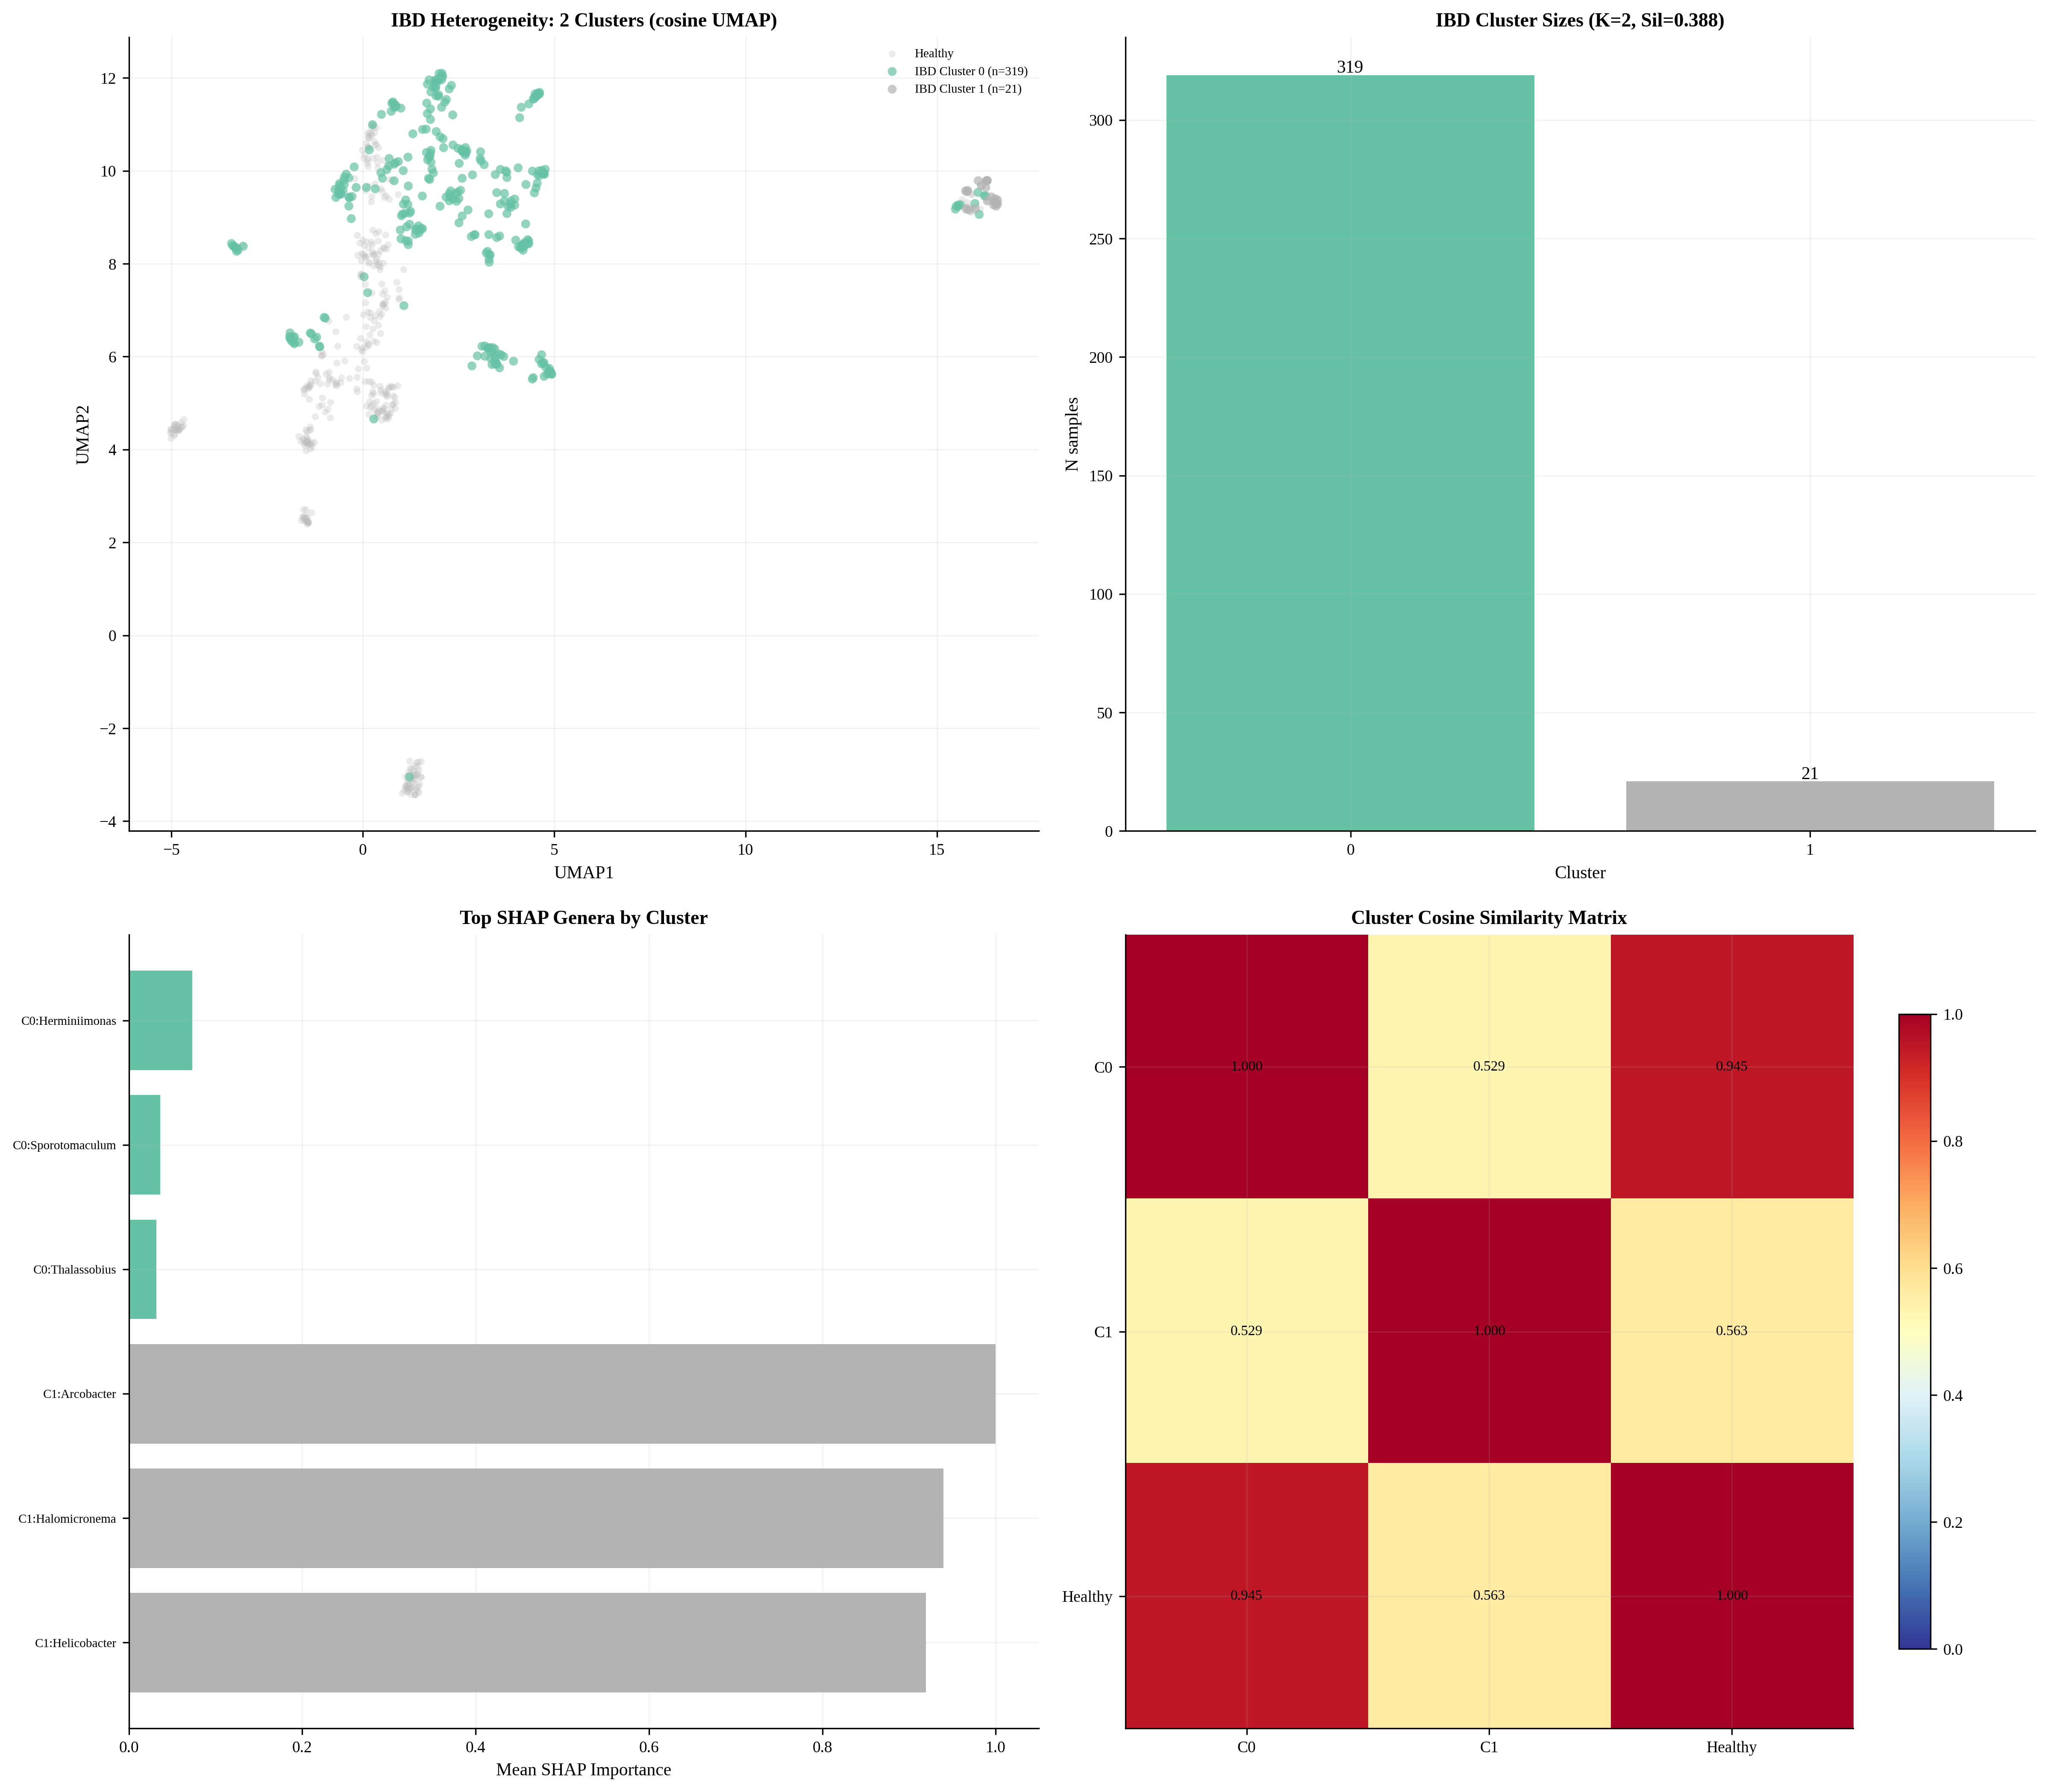
\includegraphics[width=0.95\textwidth]{figures/phase35_heterogeneity.png}
\caption{\textbf{IBD heterogeneity analysis.}
(A) UMAP with IBD clusters colored separately from healthy samples. (B) Cluster sizes
with silhouette score. (C) Top LOO-attributed genera per cluster. (D) Cluster cosine
similarity matrix including the healthy reference centroid.}
\label{fig:heterogeneity}
\end{figure}

\begin{figure}[ht]
\centering
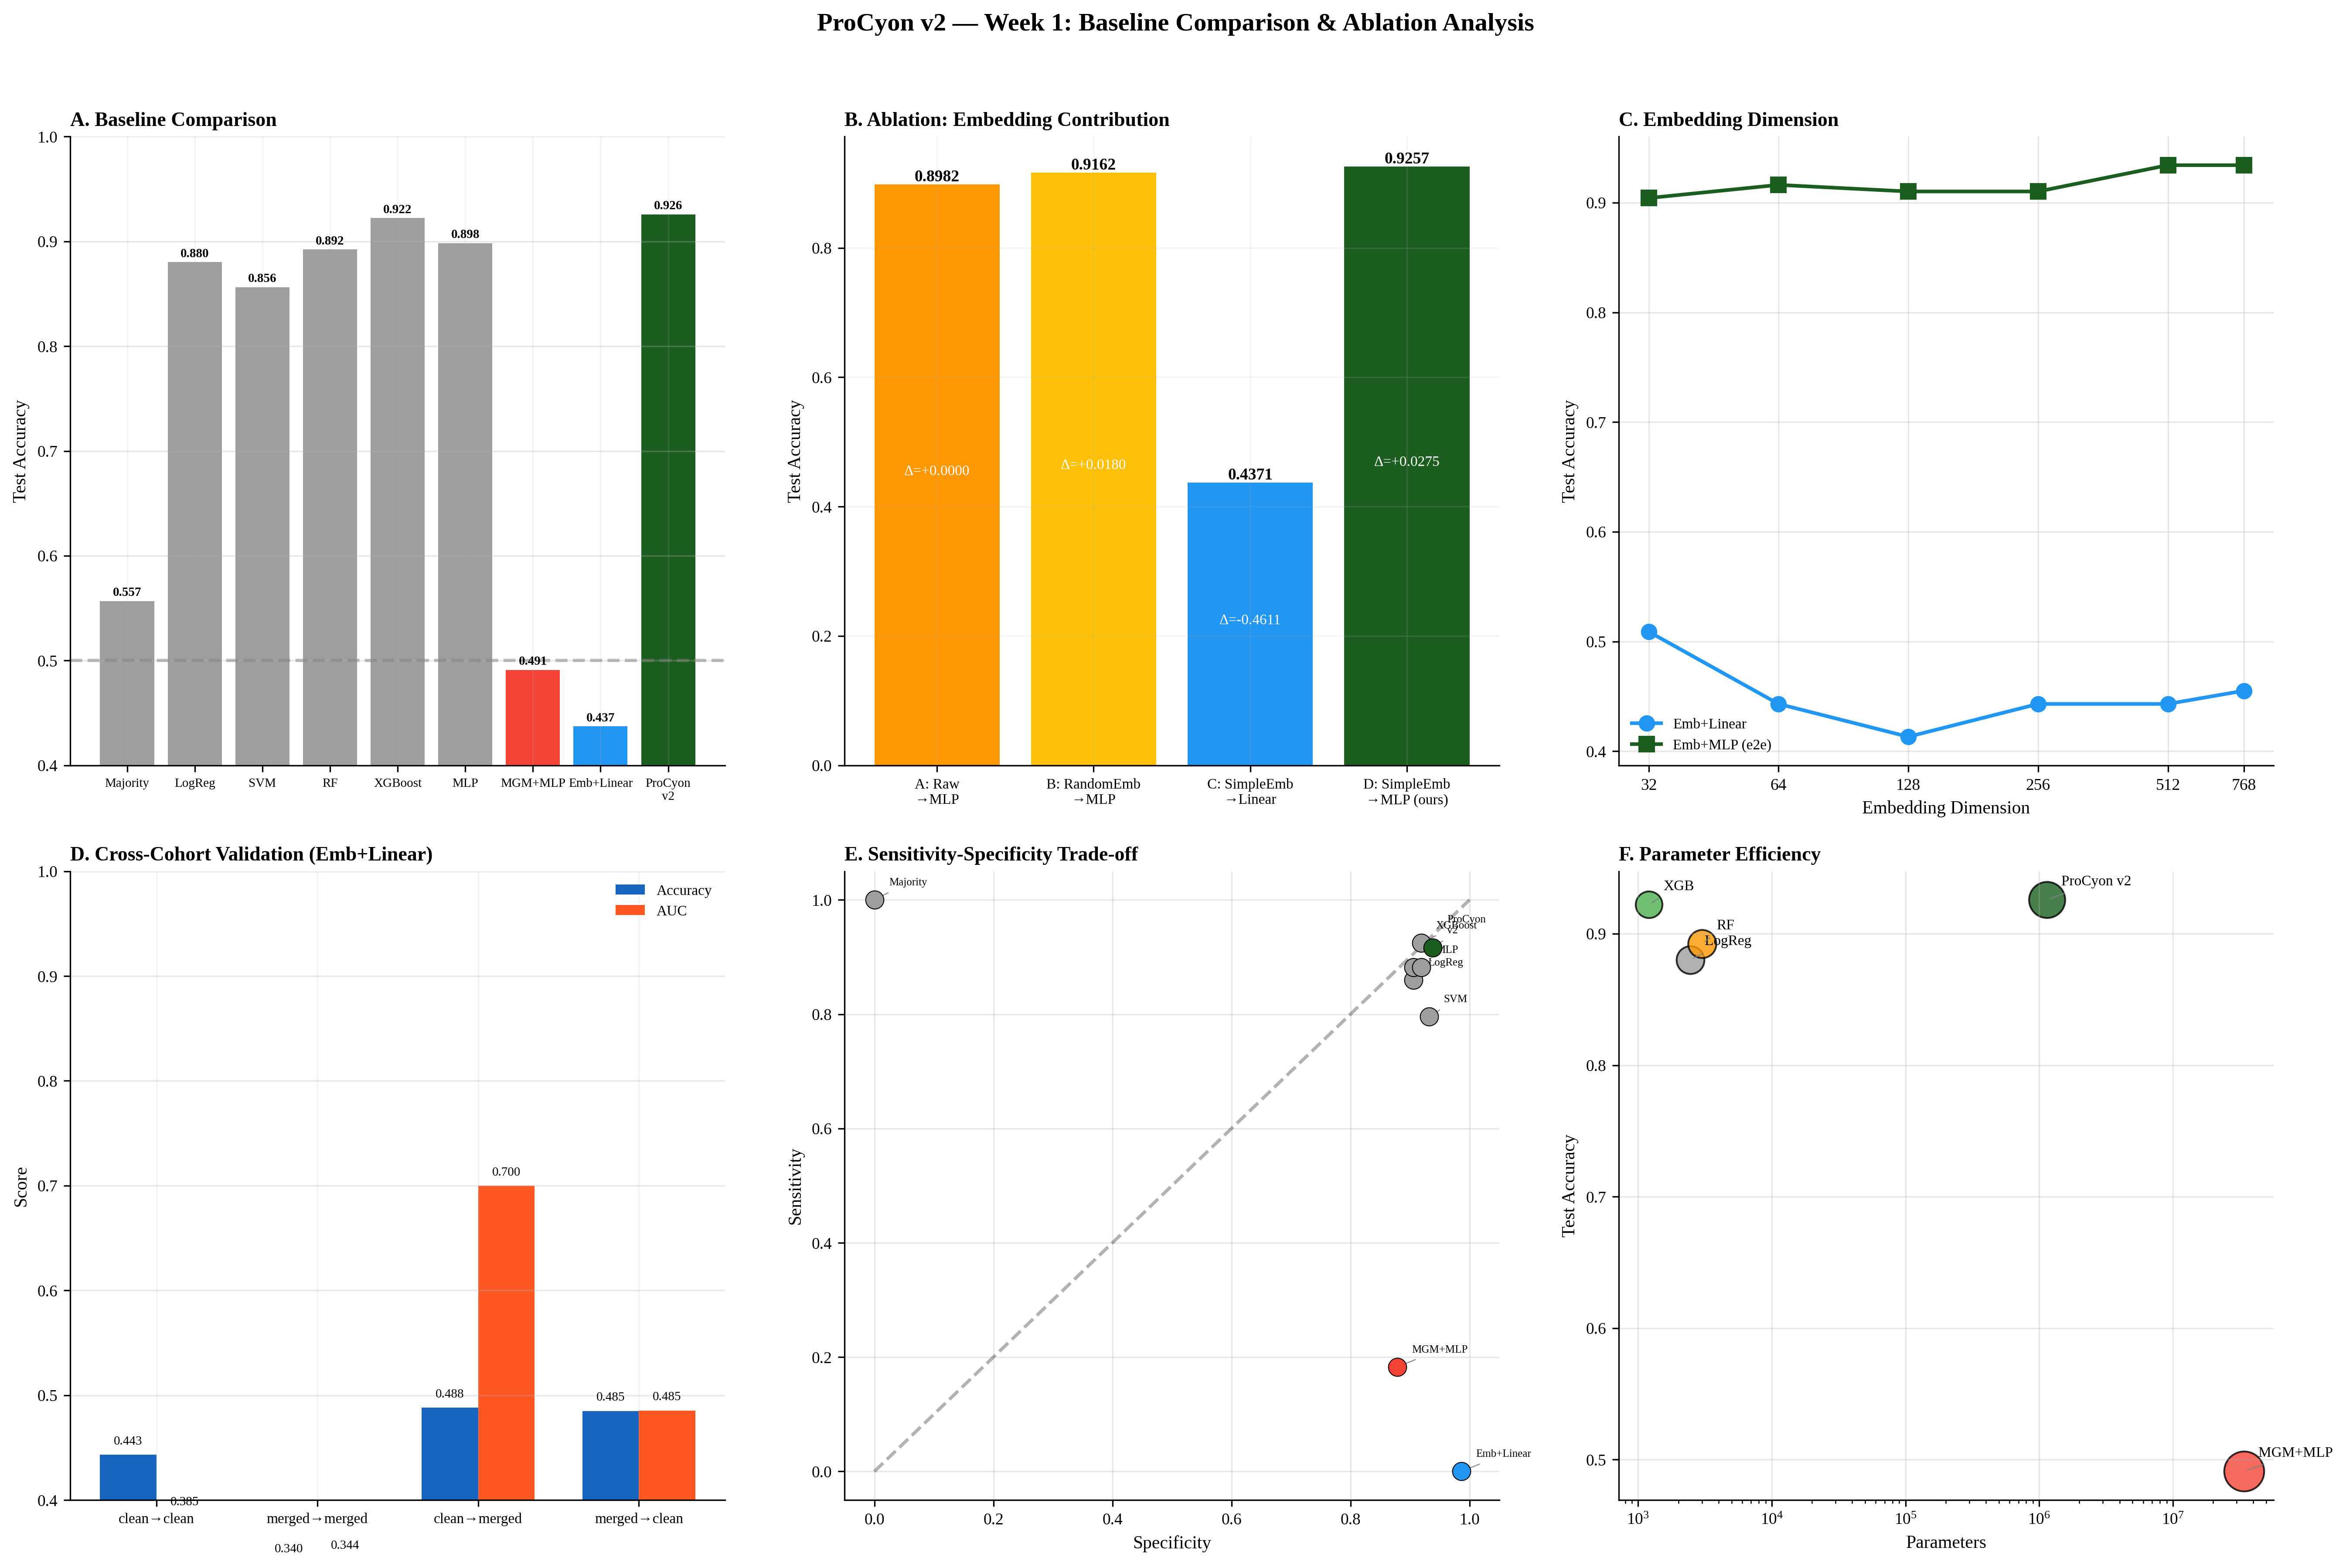
\includegraphics[width=0.95\textwidth]{figures/week1_figure.png}
\caption{\textbf{Comprehensive comparison analysis.}
(A) Baseline accuracy comparison. (B) Ablation: embedding contribution. (C) Embedding
dimension sweep. (D) Cross-dataset transfer. (E) Sensitivity--specificity trade-off.
(F) Parameter efficiency.}
\label{fig:baseline}
\end{figure}

\begin{table}[ht]
\centering
\caption{\textbf{Ablation: contribution of each architectural component.}
All variants use the identical MLP architecture. $\Delta$ shows improvement over variant A.}
\label{tab:ablation}
\begin{tabular}{lcccccc}
\toprule
\textbf{Variant} & \textbf{ACC} & \textbf{AUC} & \textbf{Prec.} & \textbf{Rec.} & \textbf{F1} & \textbf{$\Delta$ACC} \\
\midrule
A: Raw$\rightarrow$MLP & 0.8982 & 0.9605 & 0.9318 & 0.8817 & 0.9061 & --- \\
B: RandomEmb$\rightarrow$MLP & 0.9162 & 0.9762 & 0.9341 & 0.9140 & 0.9239 & +1.80\% \\
C: SimpleEmb$\rightarrow$Linear & 0.4431 & 0.3362 & 0.5000 & 0.0645 & 0.1143 & $-$45.51\% \\
D: \textbf{SimpleEmb$\rightarrow$MLP} & \textbf{0.9257} & \textbf{0.9750} & \textbf{0.9451} & \textbf{0.9161} & \textbf{0.9348} & \textbf{+2.75\%} \\
\bottomrule
\end{tabular}
\end{table}

\begin{table}[ht]
\centering
\caption{\textbf{Representation and head ablation under grouped-CV (15 folds).}
Presence = multi-hot token presence vector; Embedding64 = trainable $E{=}64$ embedding + masked mean pool.}
\label{tab:repr_ablation}
\begin{tabular}{lcccc}
\toprule
\textbf{Model} & \textbf{Params} & \textbf{ACC} & \textbf{AUROC} & \textbf{AUPRC} \\
\midrule
Presence + Linear & 2,454 & 0.876 $\pm$ 0.037 & 0.949 $\pm$ 0.019 & 0.957 $\pm$ 0.018 \\
Presence + MLP & 315,138 & \textbf{0.912} $\pm$ 0.025 & \textbf{0.969} $\pm$ 0.012 & \textbf{0.973} $\pm$ 0.012 \\
Embedding64 + Linear & 78,594 & 0.857 $\pm$ 0.036 & 0.916 $\pm$ 0.029 & 0.909 $\pm$ 0.049 \\
Embedding64 + MLP (ours) & 96,130 & 0.906 $\pm$ 0.021 & 0.956 $\pm$ 0.016 & 0.954 $\pm$ 0.031 \\
\bottomrule
\end{tabular}
\end{table}

\begin{table}[ht]
\centering
\caption{\textbf{Embedding dimension ablation under the exact input-grouped 3$\times$5-fold CV protocol.}
Only the embedding dimension changes; all other architecture and optimization settings are fixed.
Held-out test set results are shown for reference in parentheses.}
\label{tab:embedding}
\begin{tabular}{lcccccr}
\toprule
\textbf{$E$} & \textbf{Params} & \textbf{ACC} & \textbf{Macro-F1} & \textbf{AUROC} & \textbf{AUPRC} \\
\midrule
16  & 24,994 & 0.855 $\pm$ 0.027 & 0.854 $\pm$ 0.027 & 0.924 $\pm$ 0.020 & 0.918 $\pm$ 0.041 \\
32  & 48,706 & 0.879 $\pm$ 0.033 & 0.878 $\pm$ 0.034 & 0.941 $\pm$ 0.019 & 0.944 $\pm$ 0.022 \\
64  & 96,130 & 0.906 $\pm$ 0.021 & 0.905 $\pm$ 0.021 & 0.956 $\pm$ 0.016 & 0.954 $\pm$ 0.031 \\
128 & 190,978 & 0.908 $\pm$ 0.024 & 0.907 $\pm$ 0.024 & 0.957 $\pm$ 0.015 & 0.956 $\pm$ 0.026 \\
256 & 380,674 & 0.909 $\pm$ 0.020 & 0.909 $\pm$ 0.020 & 0.956 $\pm$ 0.015 & 0.952 $\pm$ 0.037 \\
\textbf{512} & \textbf{760,066} & \textbf{0.914} $\pm$ 0.020 & \textbf{0.913} $\pm$ 0.019 & \textbf{0.957} $\pm$ 0.014 & 0.952 $\pm$ 0.032 \\
768 & 1,139,458 & \textbf{0.914} $\pm$ 0.016 & \textbf{0.913} $\pm$ 0.016 & 0.957 $\pm$ 0.015 & 0.952 $\pm$ 0.035 \\
\bottomrule
\end{tabular}
\end{table}

\begin{table}[ht]
\centering
\caption{\textbf{Nested grouped-CV learning curves (AUROC).}
The training fraction is sampled from only the outer training groups.}
\label{tab:learning}
\begin{tabular}{lccc}
\toprule
\textbf{Train fraction} & \textbf{HGB} & \textbf{Presence+MLP} & \textbf{Embedding64+MLP (ours)} \\
\midrule
20\% & 0.922 $\pm$ 0.027 & 0.940 $\pm$ 0.019 & 0.900 $\pm$ 0.027 \\
40\% & 0.962 $\pm$ 0.012 & 0.959 $\pm$ 0.011 & 0.929 $\pm$ 0.022 \\
60\% & 0.972 $\pm$ 0.010 & 0.965 $\pm$ 0.011 & 0.947 $\pm$ 0.015 \\
80\% & 0.976 $\pm$ 0.009 & 0.966 $\pm$ 0.010 & 0.951 $\pm$ 0.017 \\
100\% & \textbf{0.979} $\pm$ 0.010 & 0.969 $\pm$ 0.012 & 0.956 $\pm$ 0.016 \\
\bottomrule
\end{tabular}
\end{table}

\begin{table}[ht]
\centering
\caption{\textbf{Structural baselines: inductive bias comparison.}
All models trained on identical data without pretraining (except MGM).
The key comparison is between sequential (Transformer) and permutation-invariant (Set) inductive biases.}
\label{tab:structural}
\begin{tabular}{lp{4.0cm}cccc}
\toprule
\textbf{Model} & \textbf{Inductive Bias} & \textbf{Pretrain} & \textbf{ACC} & \textbf{AUC} & \textbf{Params} \\
\midrule
Raw + MLP & None (tabular) & \ding{55} & 0.8982 & 0.9605 & 330K \\
FT-Transformer & Sequential & \ding{55} & 0.9102 & 0.9552 & 769K \\
MGM & Sequential & \ding{51} & 0.5090 & 0.4625 & 34M \\
\midrule
DeepSets & Permutation-invariant & \ding{55} & \textbf{0.9162} & \textbf{0.9731} & 512K \\
\textbf{SimpleEmb} & \textbf{Permutation-invariant + Embedding} & \ding{55} & \textbf{0.9162} & 0.9640 & 347K \\
\bottomrule
\end{tabular}
\end{table}

\begin{figure}[ht]
\centering
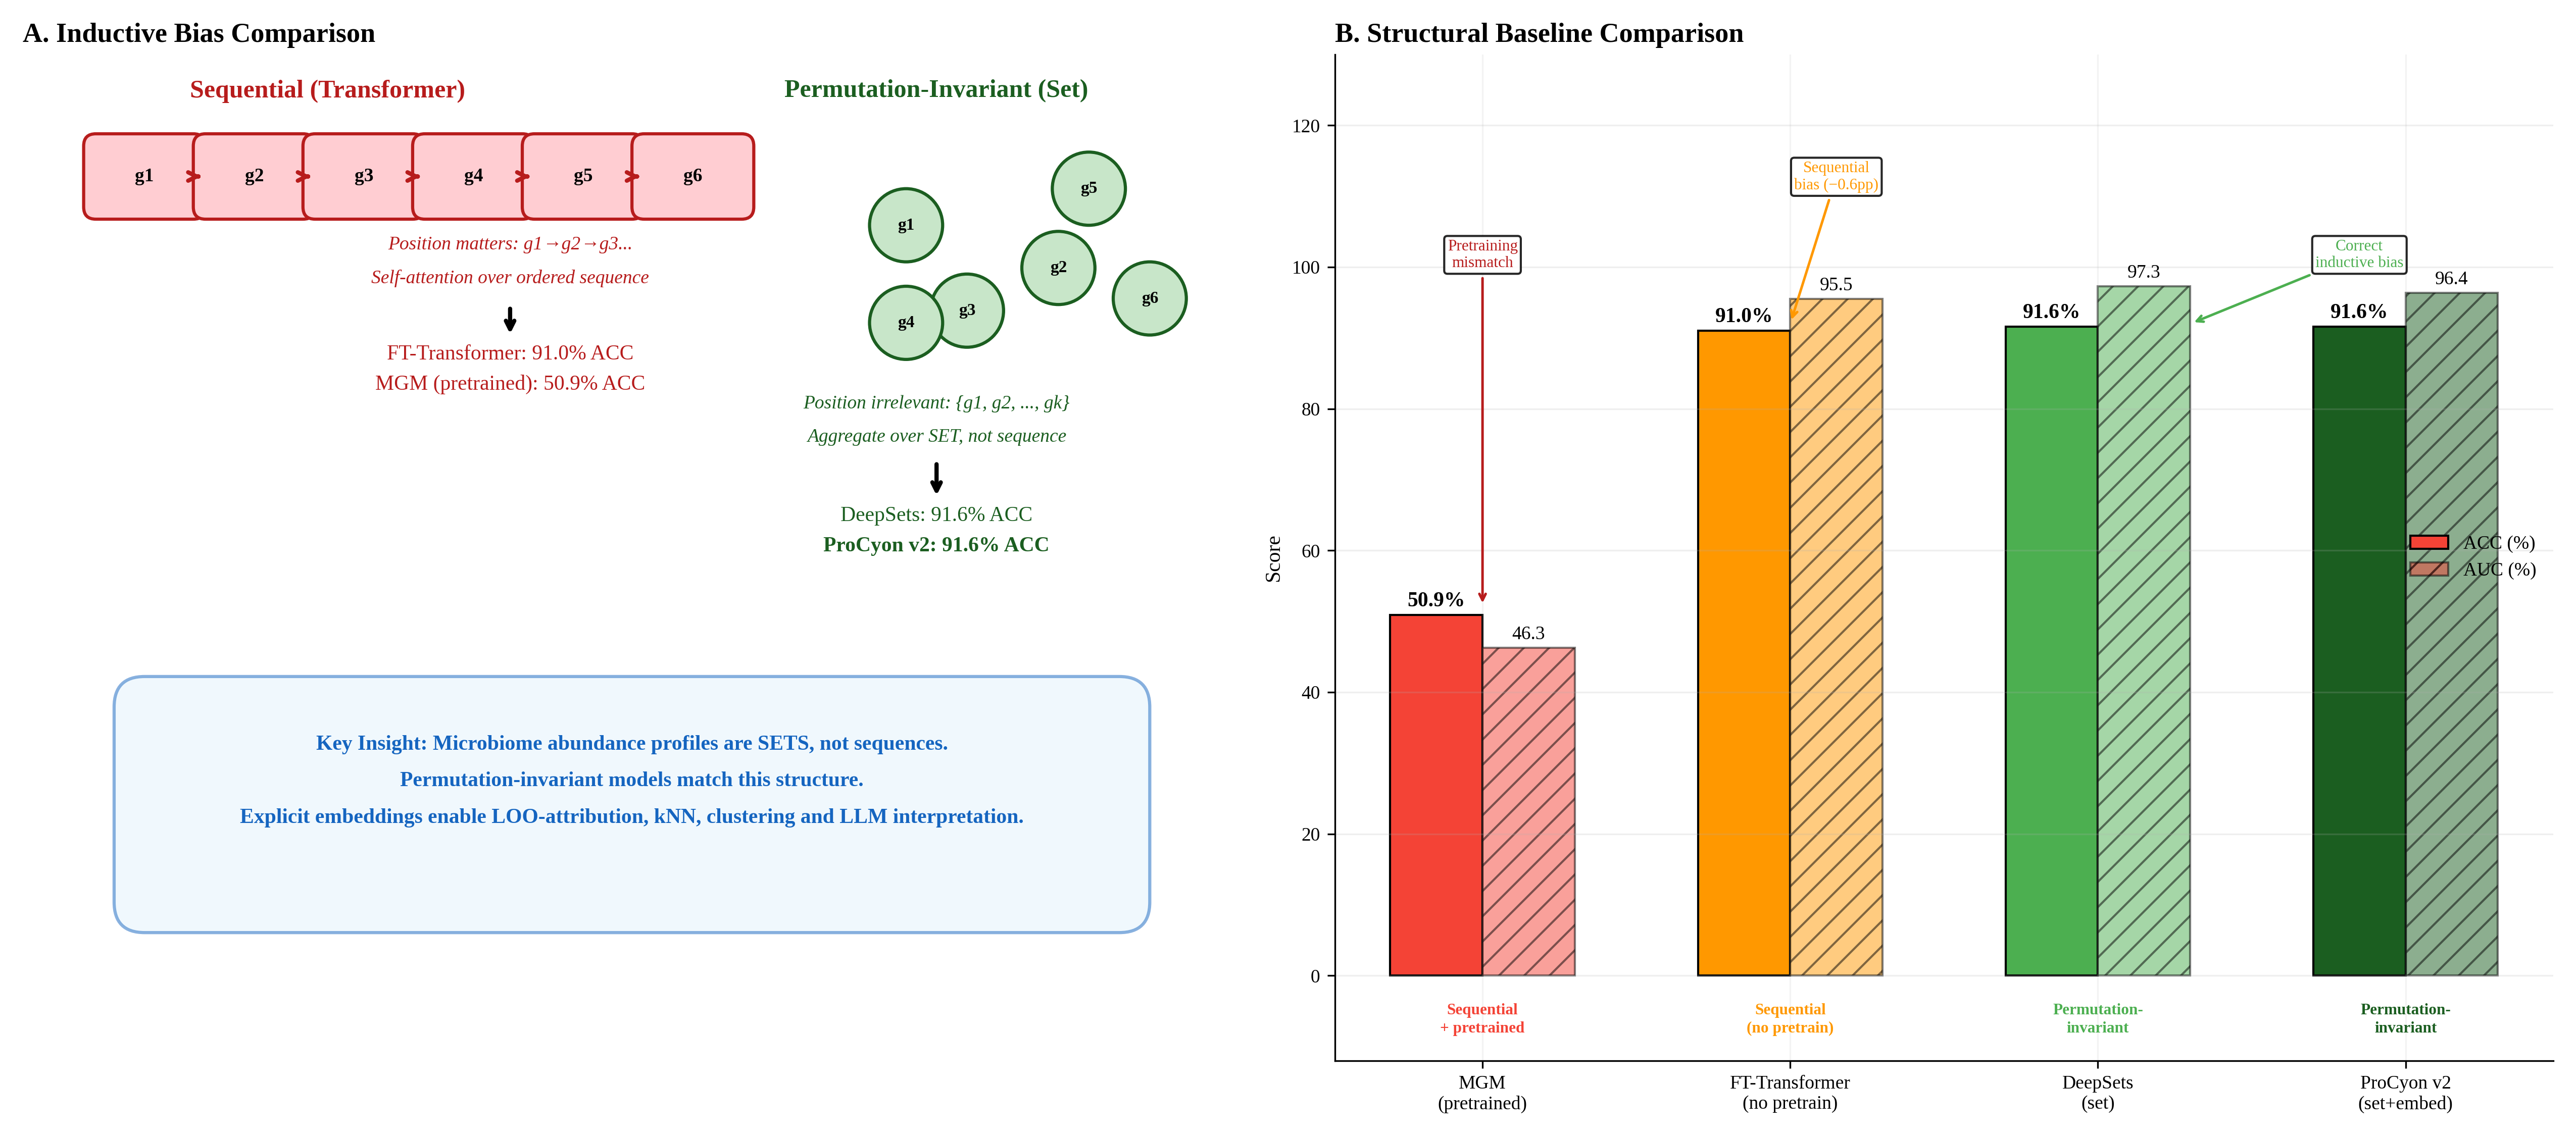
\includegraphics[width=0.95\textwidth]{figures/inductive_bias_figure.png}
\caption{\textbf{Inductive bias comparison.}
(A) Sequential (Transformer) vs.\ permutation-invariant (Set) inductive biases with
corresponding model performance. (B) Structural baseline accuracy and AUROC comparison.}
\label{fig:inductive}
\end{figure}

\begin{table}[ht]
\centering
\caption{Embedding space quality metrics.}
\label{tab:repr}
\begin{tabular}{lc}
\toprule
\textbf{Metric} & \textbf{Value} \\
\midrule
kNN ($k{=}5$, cosine) test ACC & 97.0\% \\
PCA 2D explained variance & 40.4\% \\
PCA dimensions for 90\% variance & 53 \\
IBD intra-class cosine similarity & 0.54 \\
Healthy intra-class cosine similarity & 0.64 \\
UMAP silhouette score & 0.23 \\
\bottomrule
\end{tabular}
\end{table}

\begin{figure}[ht]
\centering
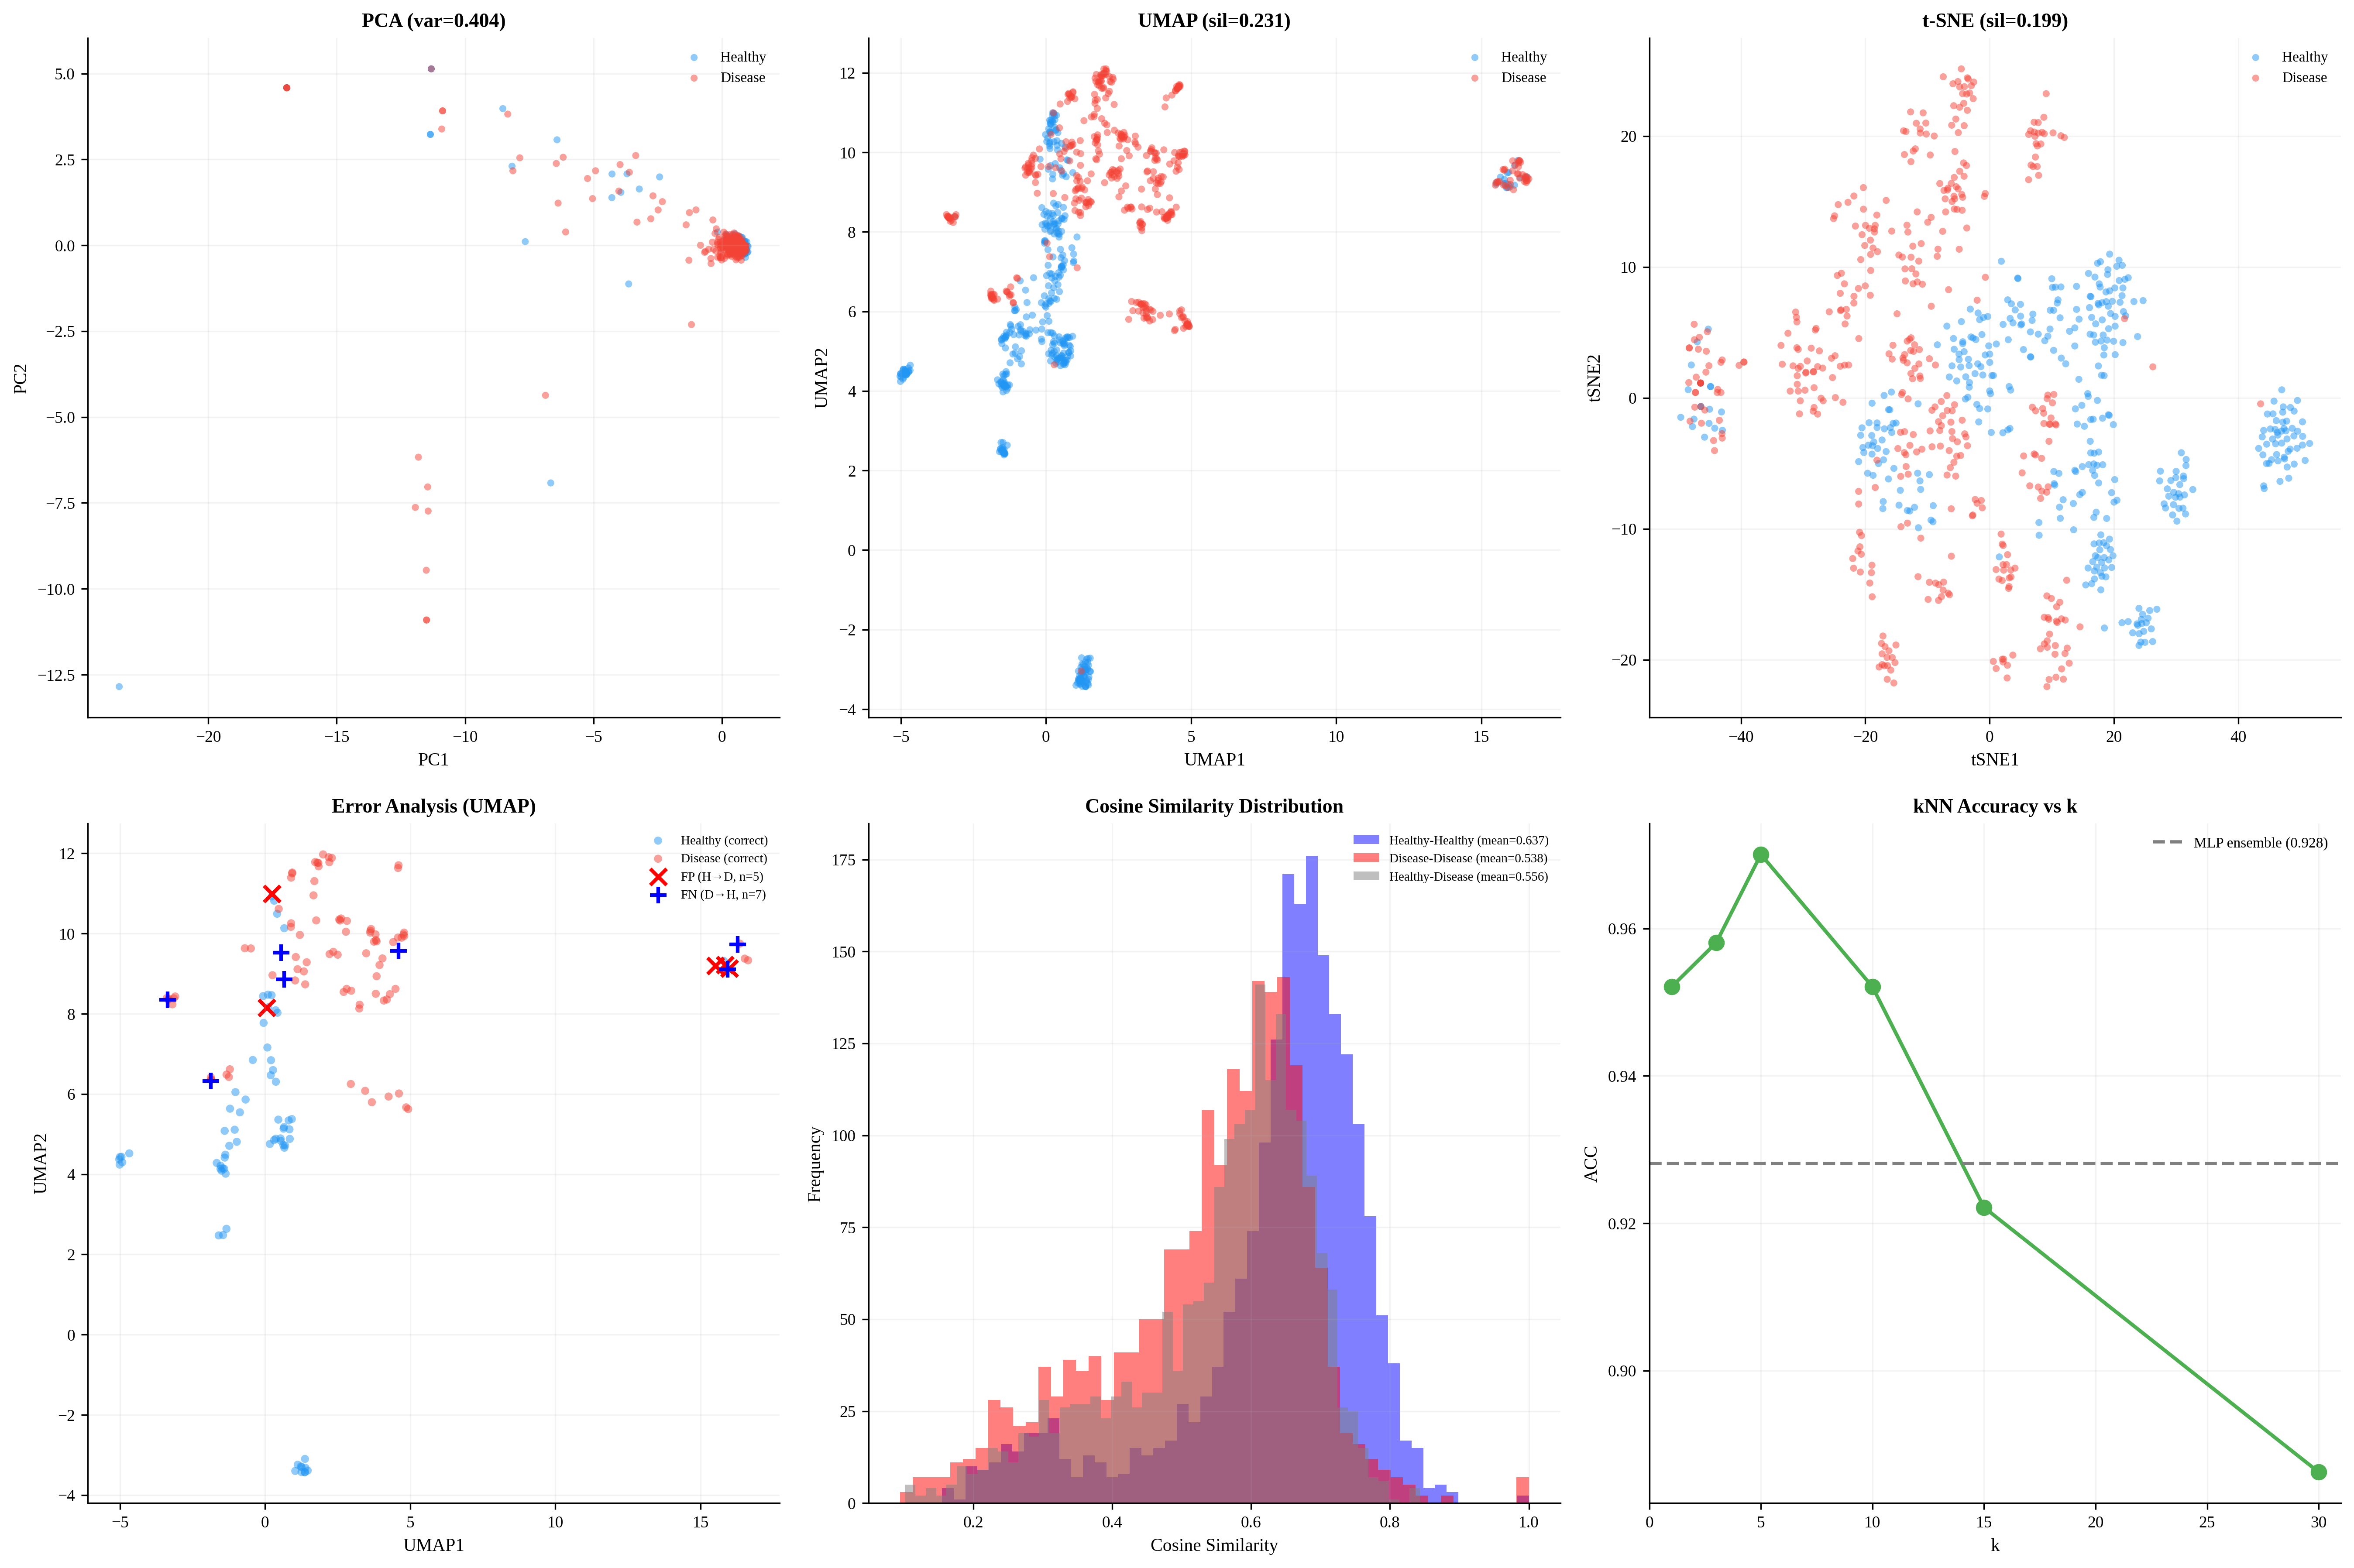
\includegraphics[width=0.95\textwidth]{figures/phase1_representation_analysis.png}
\caption{\textbf{Representation space analysis.}
(A) PCA 2D projection. (B) UMAP projection (cosine metric). (C) t-SNE projection.
(D) Prediction error analysis. (E) Intra-class cosine similarity. (F) kNN classification accuracy.}
\label{fig:repr}
\end{figure}

\begin{figure}[ht]
\centering
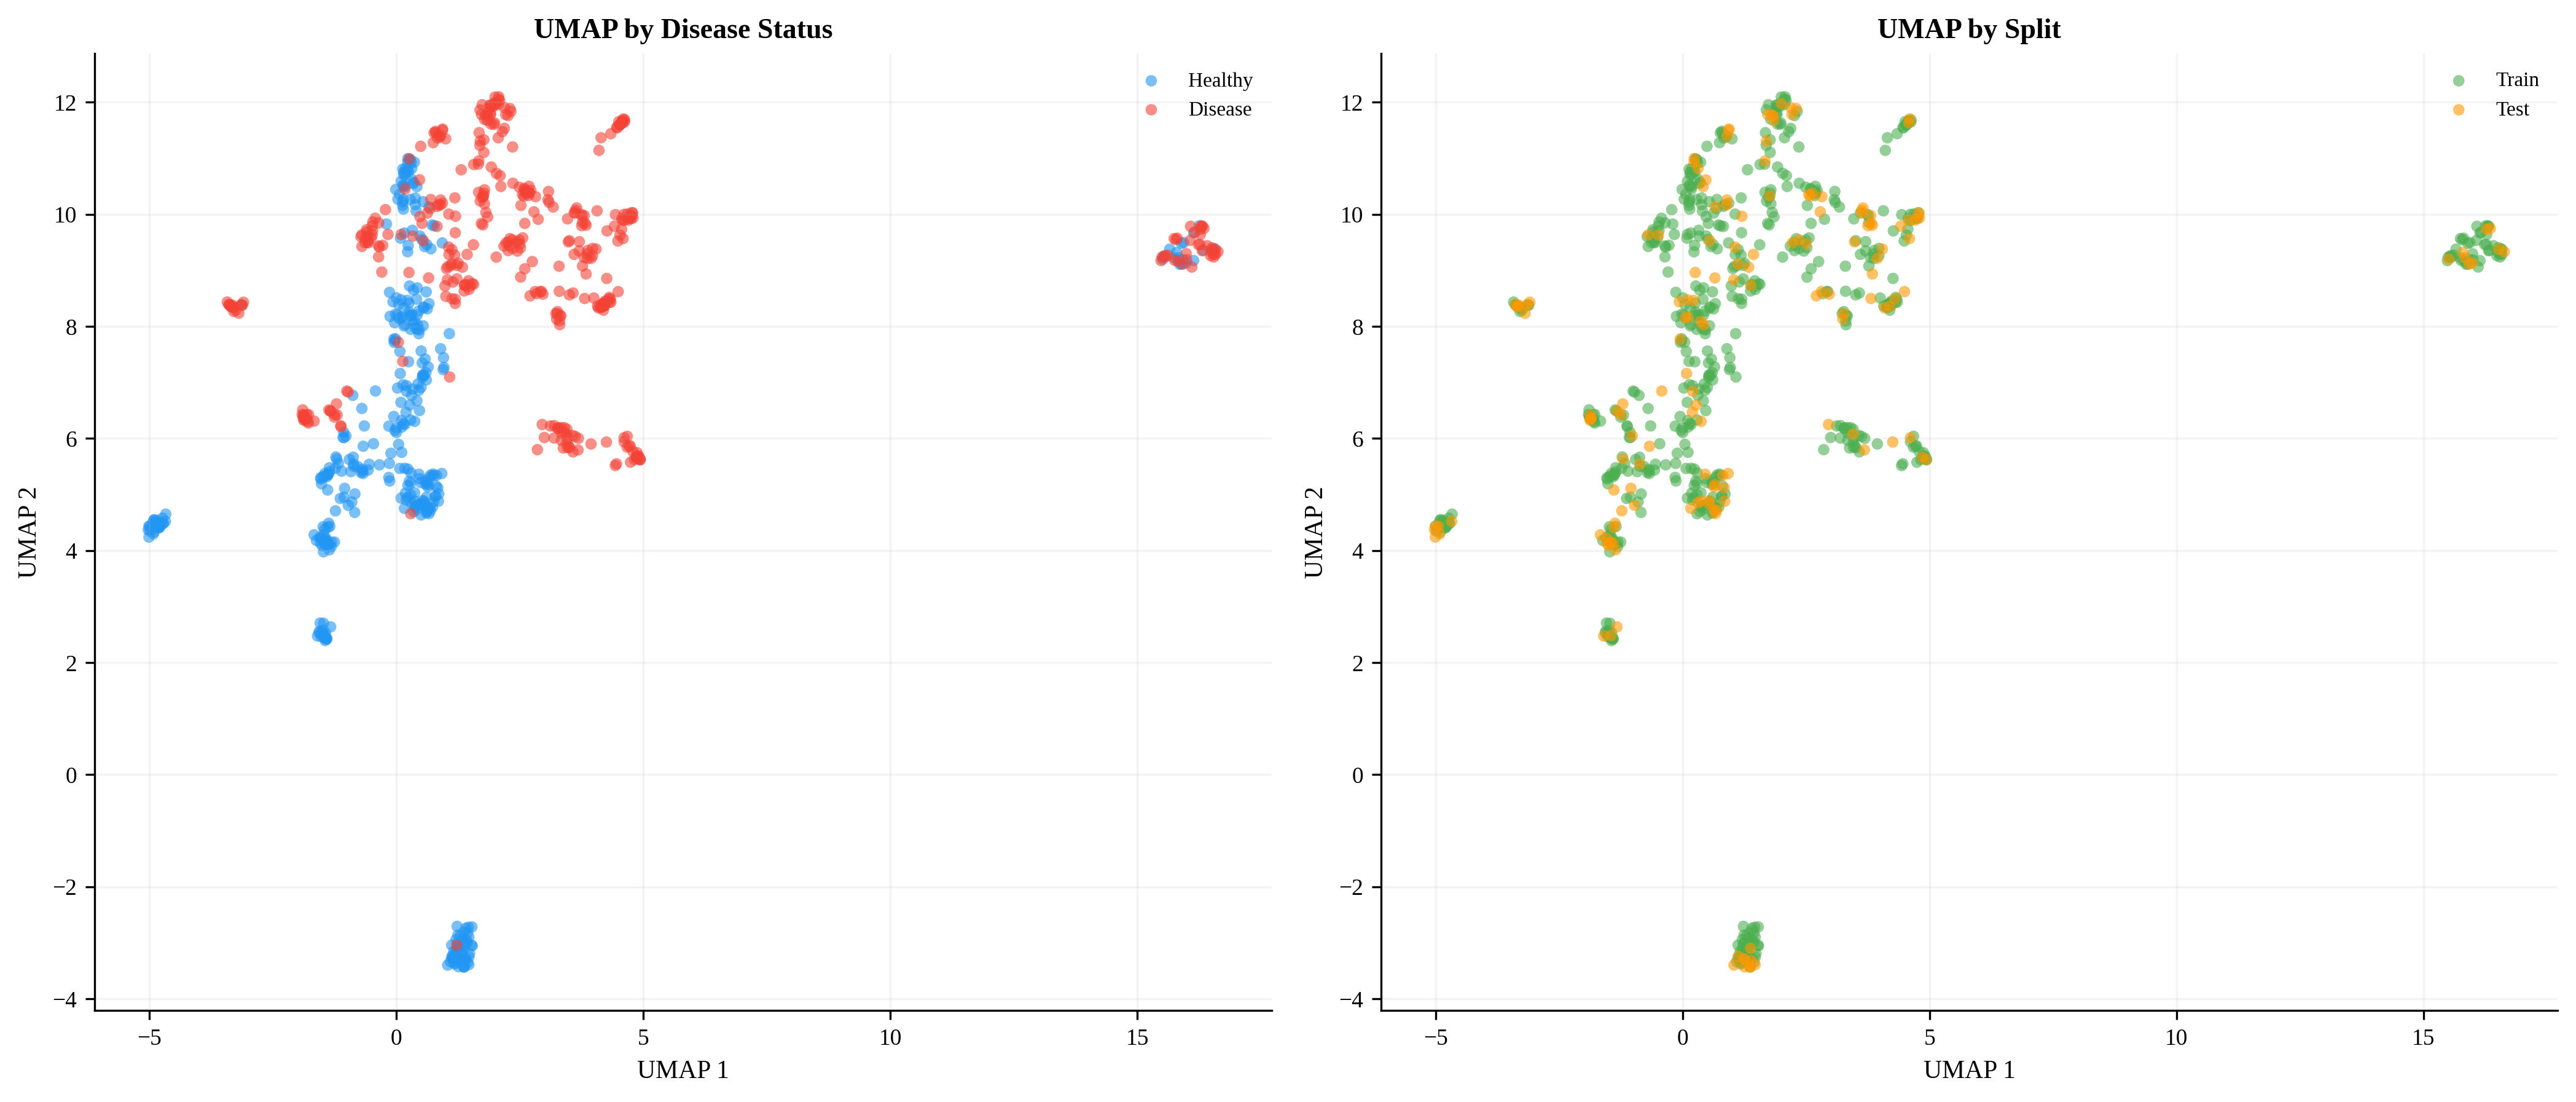
\includegraphics[width=0.75\textwidth]{figures/umap_visualization.png}
\caption{\textbf{UMAP visualization of learned embeddings.}
Disease and healthy samples in the 2D UMAP projection of the 768-dimensional embedding space.}
\label{fig:umap}
\end{figure}

\begin{table}[ht]
\centering
\caption{\textbf{LOO Attribution Reliability analysis across 5 folds.}}
\label{tab:loo}
\begin{tabular}{lc}
\toprule
\textbf{Metric} & \textbf{Value} \\
\midrule
Spearman $\rho$ (mean across fold pairs) & 0.72 ($p{<}0.001$) \\
Top-50 Jaccard (mean) & 0.07 \\
Deletion test (top-50 AUC drop) & 0.039 (vs 0.007 random) \\
Permutation control (mean $|$LOO$|$) & real 0.0096 vs.\ shuffled 0.0705 \\
Literature direction agreement & 5/6 (83.3\%) \\
Prevalence-importance correlation & $r{=}0.05$ ($p{>}0.05$) \\
\bottomrule
\end{tabular}
\end{table}

\begin{figure}[ht]
\centering

\includegraphics[width=0.95\textwidth]{figures/paper_figure_shap_analysis.png}
\caption{\textbf{Comprehensive LOO attribution analysis.}
(A) Global importance ranking (top-50 genera, color-coded by literature agreement).
(B) Prevalence vs.\ importance. (C) Cross-validation stability (Jaccard).
(D) Cluster-specific biomarker profiles. (E) Literature direction validation.
(F) Signal quality: real vs.\ permuted-label importance.}
\label{fig:loo_analysis}
\end{figure}

\begin{figure}[ht]
\centering
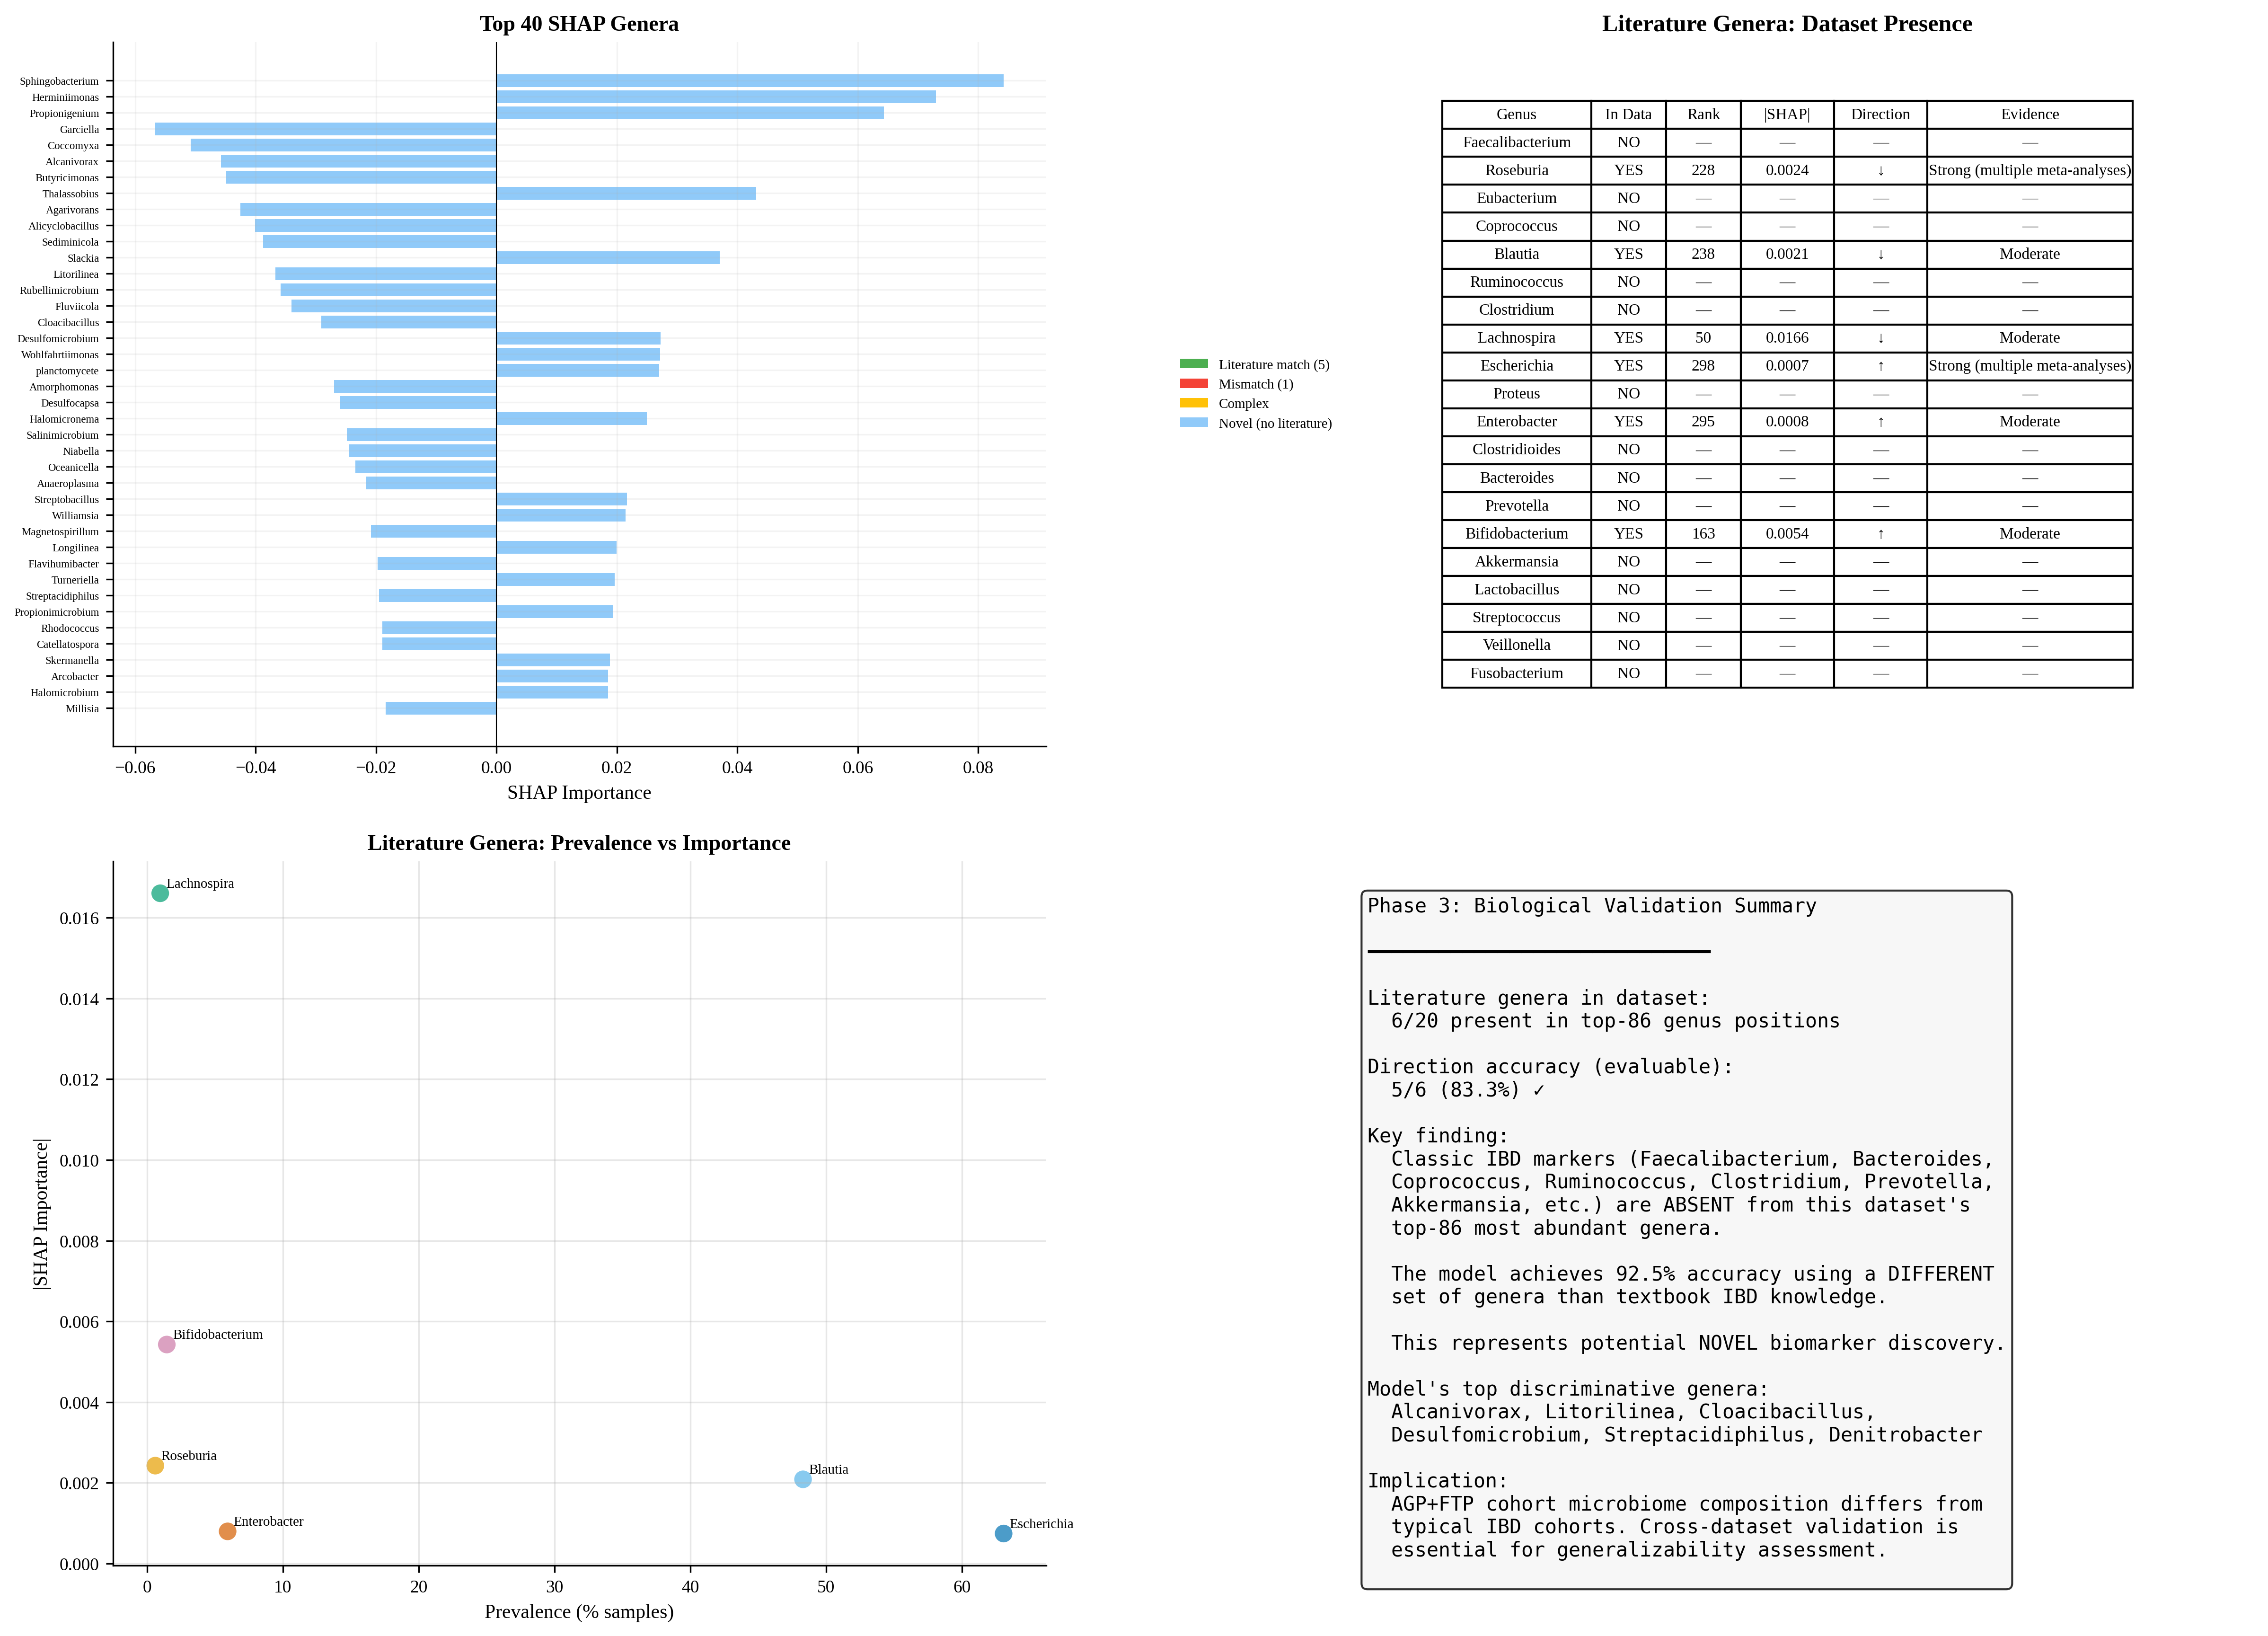
\includegraphics[width=0.9\textwidth]{figures/phase3_biological_validation.png}
\caption{\textbf{Biological validation against literature.}
Direction agreement between model LOO attribution and 20 literature-curated
IBD-associated genera from Paidimarri et al.\ (2024).}
\label{fig:literature}
\end{figure}

\begin{figure}[ht]
\centering
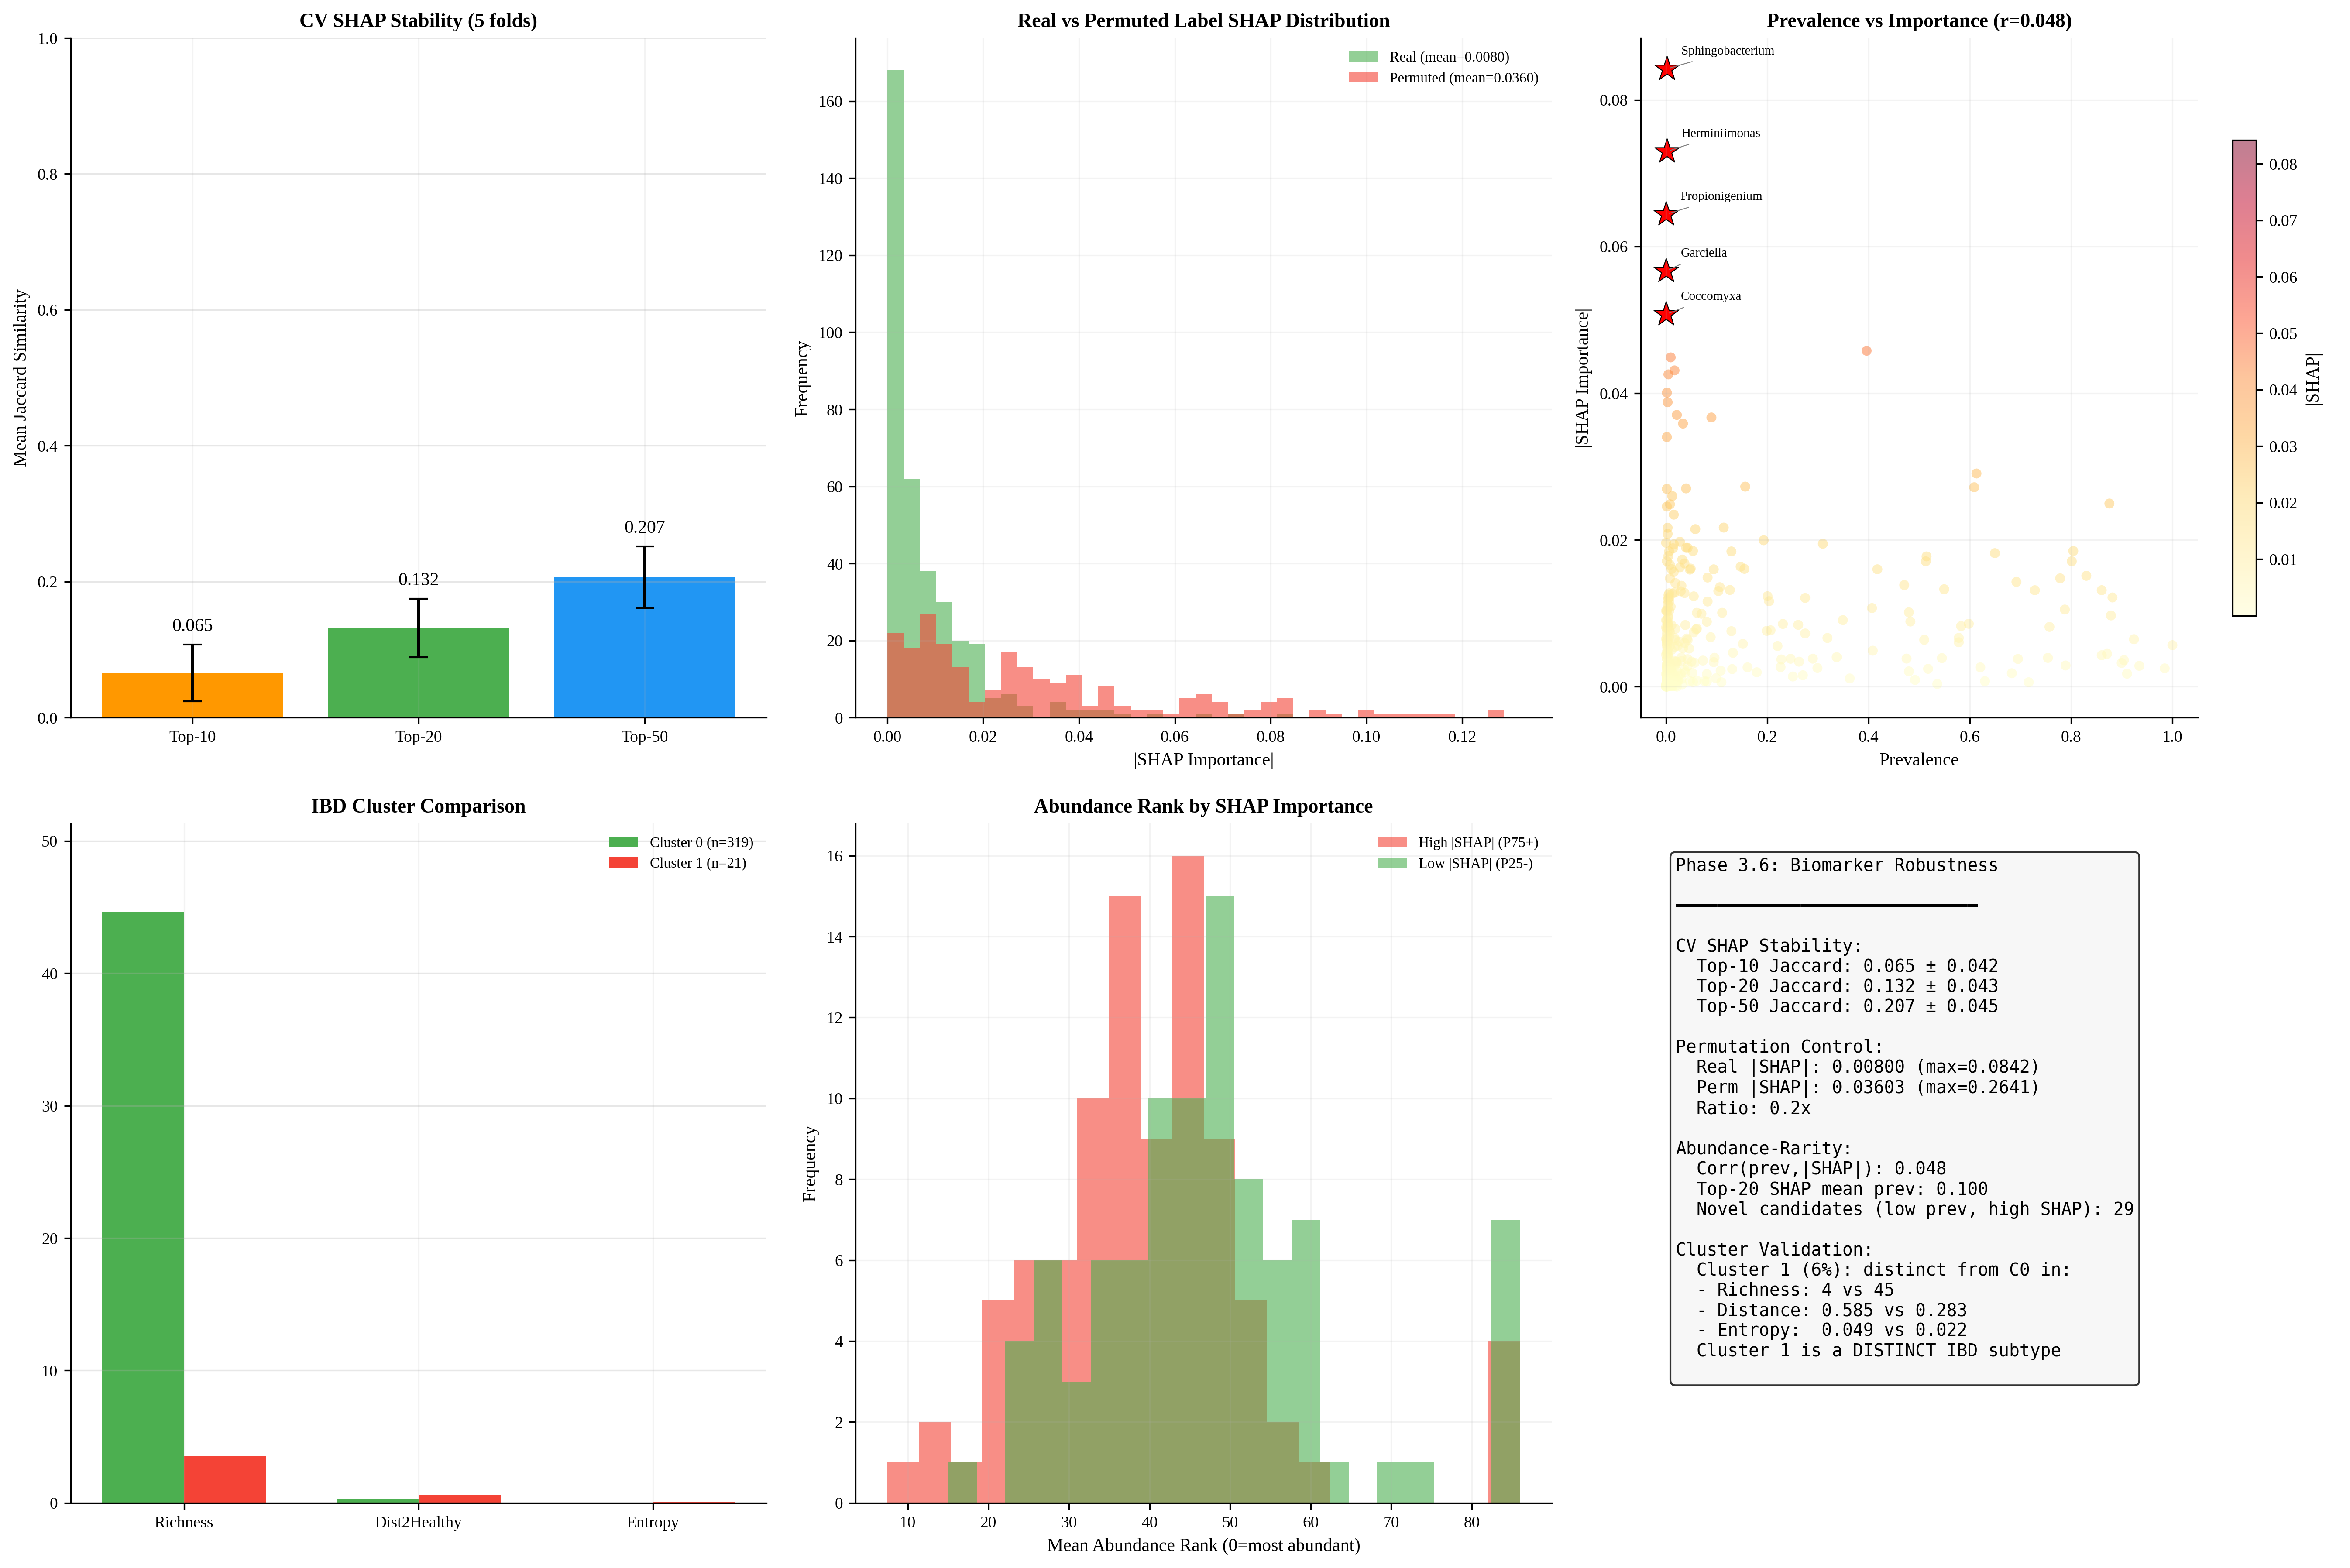
\includegraphics[width=0.9\textwidth]{figures/phase36_robustness.png}
\caption{\textbf{Biomarker robustness analysis.}
Cross-fold consistency, permutation control, abundance-independence, and
cluster validation of LOO-attributed biomarkers.}
\label{fig:robustness}
\end{figure}

\begin{table}[ht]
\centering
\caption{\textbf{LOO attribution vs.\ differential abundance (Spearman $\rho$).}}
\label{tab:attribution_bio}
\begin{tabular}{lcc}
\toprule
\textbf{Prevalence Strata} & $\rho$ & $p$-value \\
\midrule
All genera (n$=$365) & $-$0.23 & $<$0.001 \\
Prevalence $\geq$10 (n$=$186) & 0.01 & 0.901 \\
Prevalence $\geq$50 (n$=$108) & 0.11 & 0.269 \\
Prevalence $\geq$200 (n$=$66) & 0.16 & 0.188 \\
\bottomrule
\end{tabular}
\end{table}

\begin{figure}[ht]
\centering
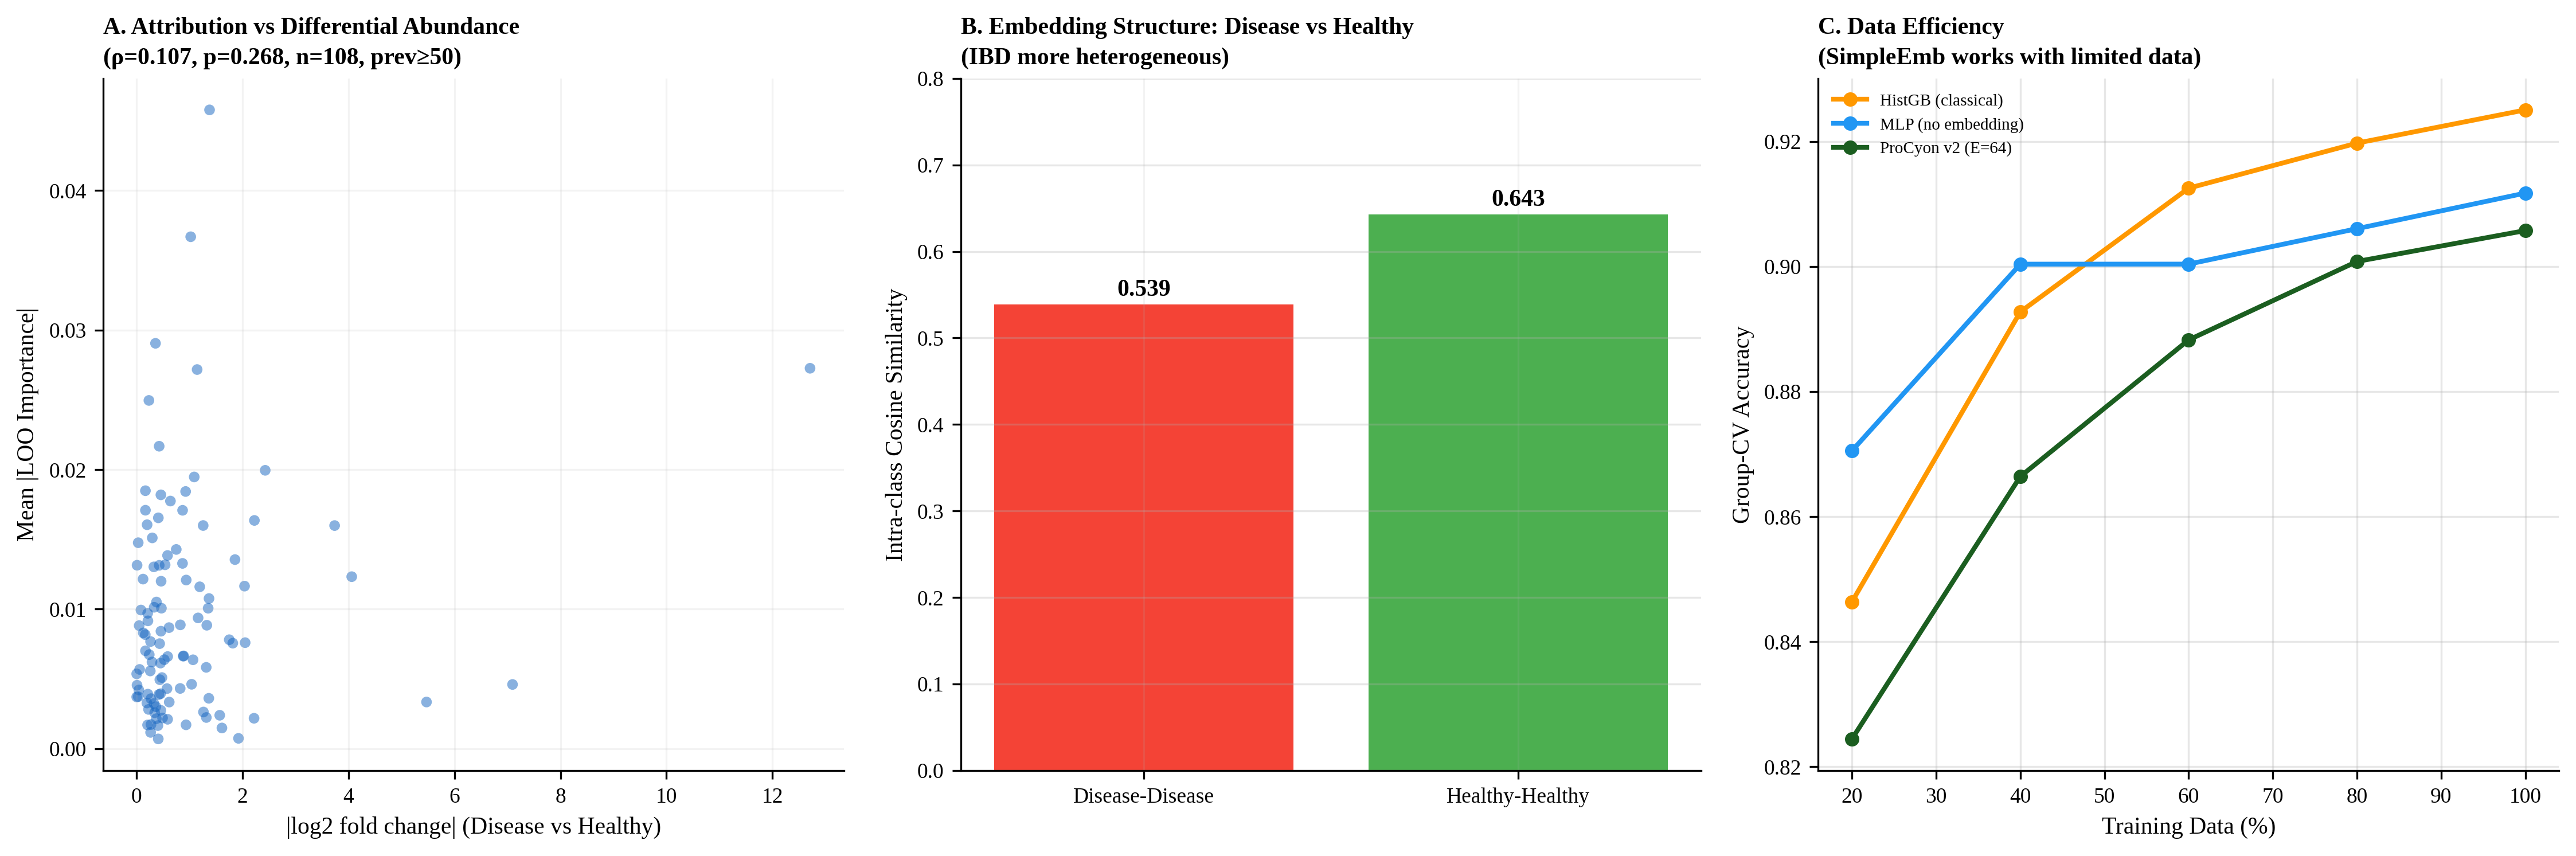
\includegraphics[width=0.95\textwidth]{figures/attribution_biology_figure.png}
\caption{\textbf{Attribution biology and embedding structure.}
(A) LOO importance vs.\ $|\log_2$ fold change$|$ scatter (prevalence $\geq$50).
(B) Intra-class cosine similarity: disease vs.\ healthy. (C) Data efficiency comparison.}
\label{fig:attribution_bio}
\end{figure}

\begin{figure}[ht]
\centering
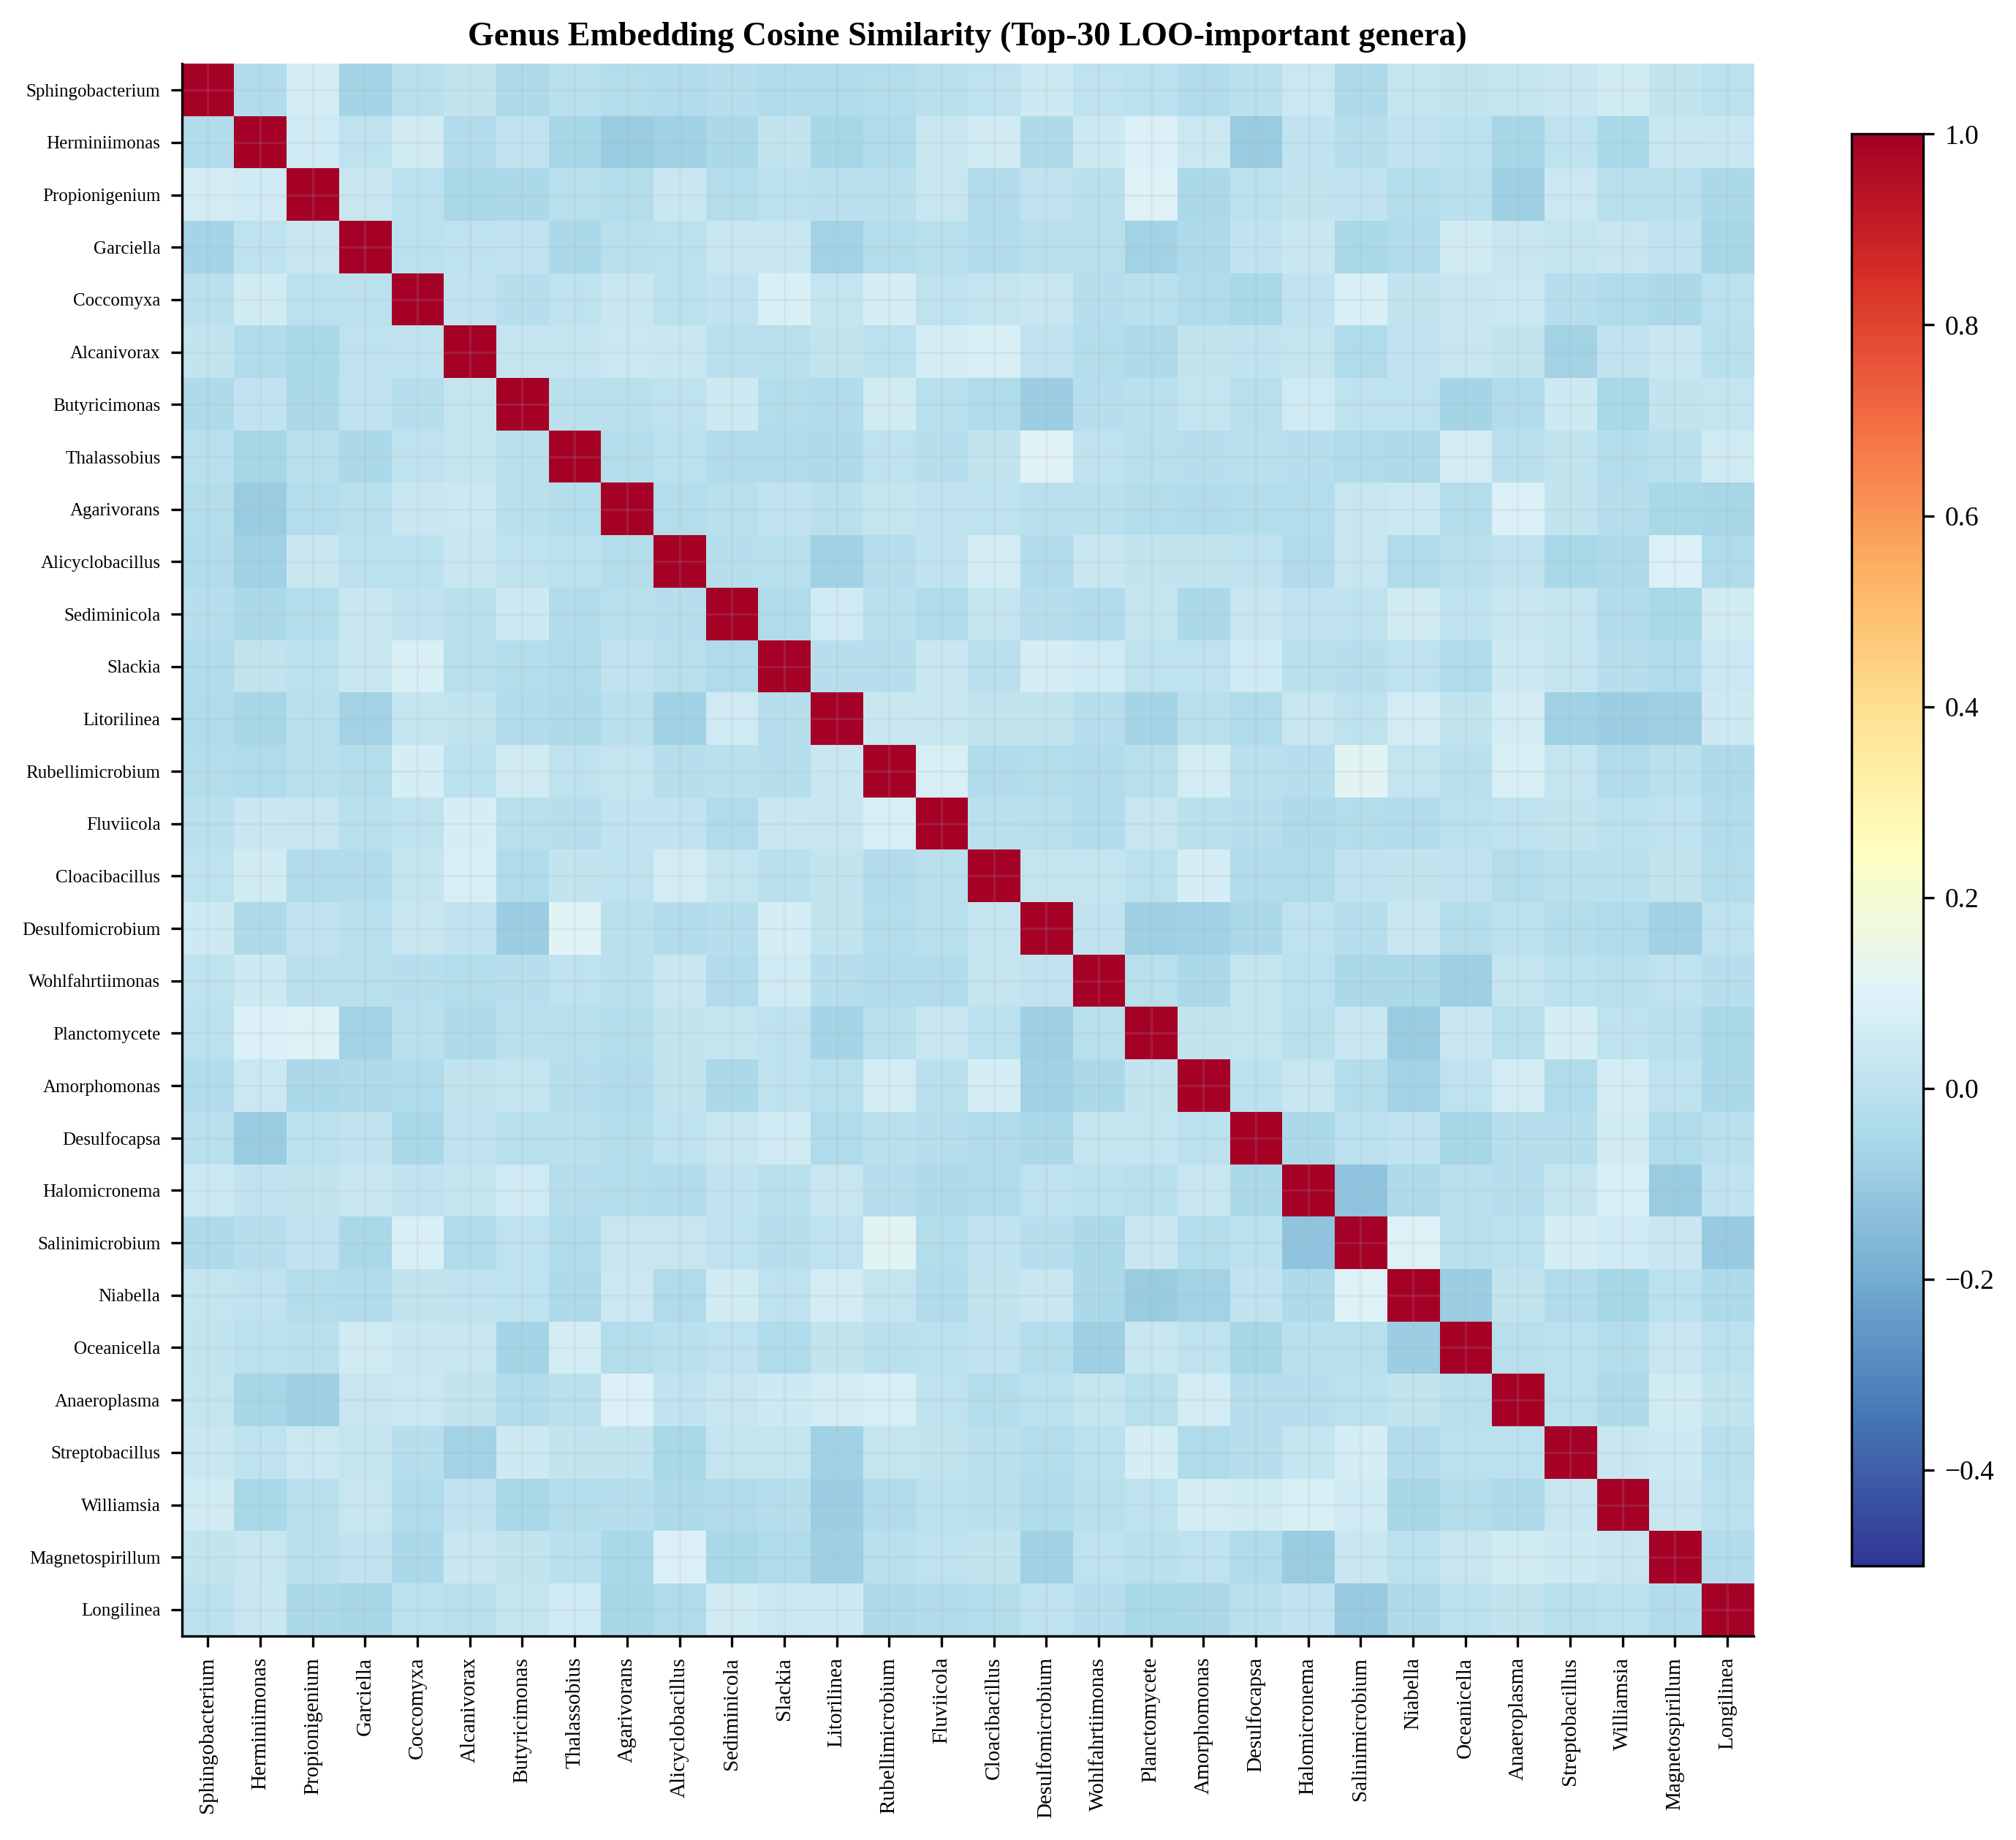
\includegraphics[width=0.75\textwidth]{figures/embedding_heatmap.png}
\caption{\textbf{Genus embedding similarity heatmap.}
Cosine similarity among the top-30 LOO-important genera in the learned embedding space.}
\label{fig:heatmap}
\end{figure}

\begin{table}[ht]
\centering
\caption{\textbf{Stratified LLM explanation quality (LOO+LLM variant, 167 samples).}}
\label{tab:llm_stratified}
\begin{tabular}{lcccc}
\toprule
\textbf{Stratum} & $n$ & \textbf{Hallucination} & \textbf{Consistency} & \textbf{Direction} \\
\midrule
Healthy samples & 74 & 0.42 & 0.97 & 0.92 \\
IBD samples & 93 & 0.31 & 0.99 & 0.95 \\
Correct predictions & 155 & 0.37 & 0.98 & 0.94 \\
Wrong predictions & 12 & 0.17 & 1.00 & 0.91 \\
\bottomrule
\end{tabular}
\end{table}

\begin{table}[ht]
\centering
\caption{\textbf{Out-of-fold case analysis (grouped split, seed 42).}
Values are disease probabilities from three models on the same held-out samples.
Extreme low-richness samples (1--4 active tokens) expose failure modes of all models.}
\label{tab:cases}
\begin{tabular}{p{3.2cm}p{2.2cm}p{1.7cm}ccc}
\toprule
\textbf{Case} & \textbf{Truth} & \textbf{Active tokens} & \textbf{\shortstack{SimpleEmb\\+MLP}} & \textbf{HGB} & \textbf{\shortstack{MGM\\+MLP}} \\
\midrule
SimpleEmb correct; HGB wrong & Healthy & 86 & H (0.003) & D (0.883) & D (0.887) \\
HGB correct; SimpleEmb wrong & Disease & 86 & H (0.104) & D (0.997) & H (0.175) \\
SimpleEmb correct; MGM wrong & Disease & 4 & D (1.000) & D (0.749) & H (0.398) \\
High-conf.\ false positive & Healthy & 1 & D (1.000) & D (0.824) & D (1.000) \\
High-conf.\ false negative & Disease & 2 & H (0.000) & D (0.749) & D (0.889) \\
All models correct & Disease & 23 & D (1.000) & D (1.000) & D (1.000) \\
\bottomrule
\end{tabular}
\end{table}

\begin{figure}[ht]
\centering
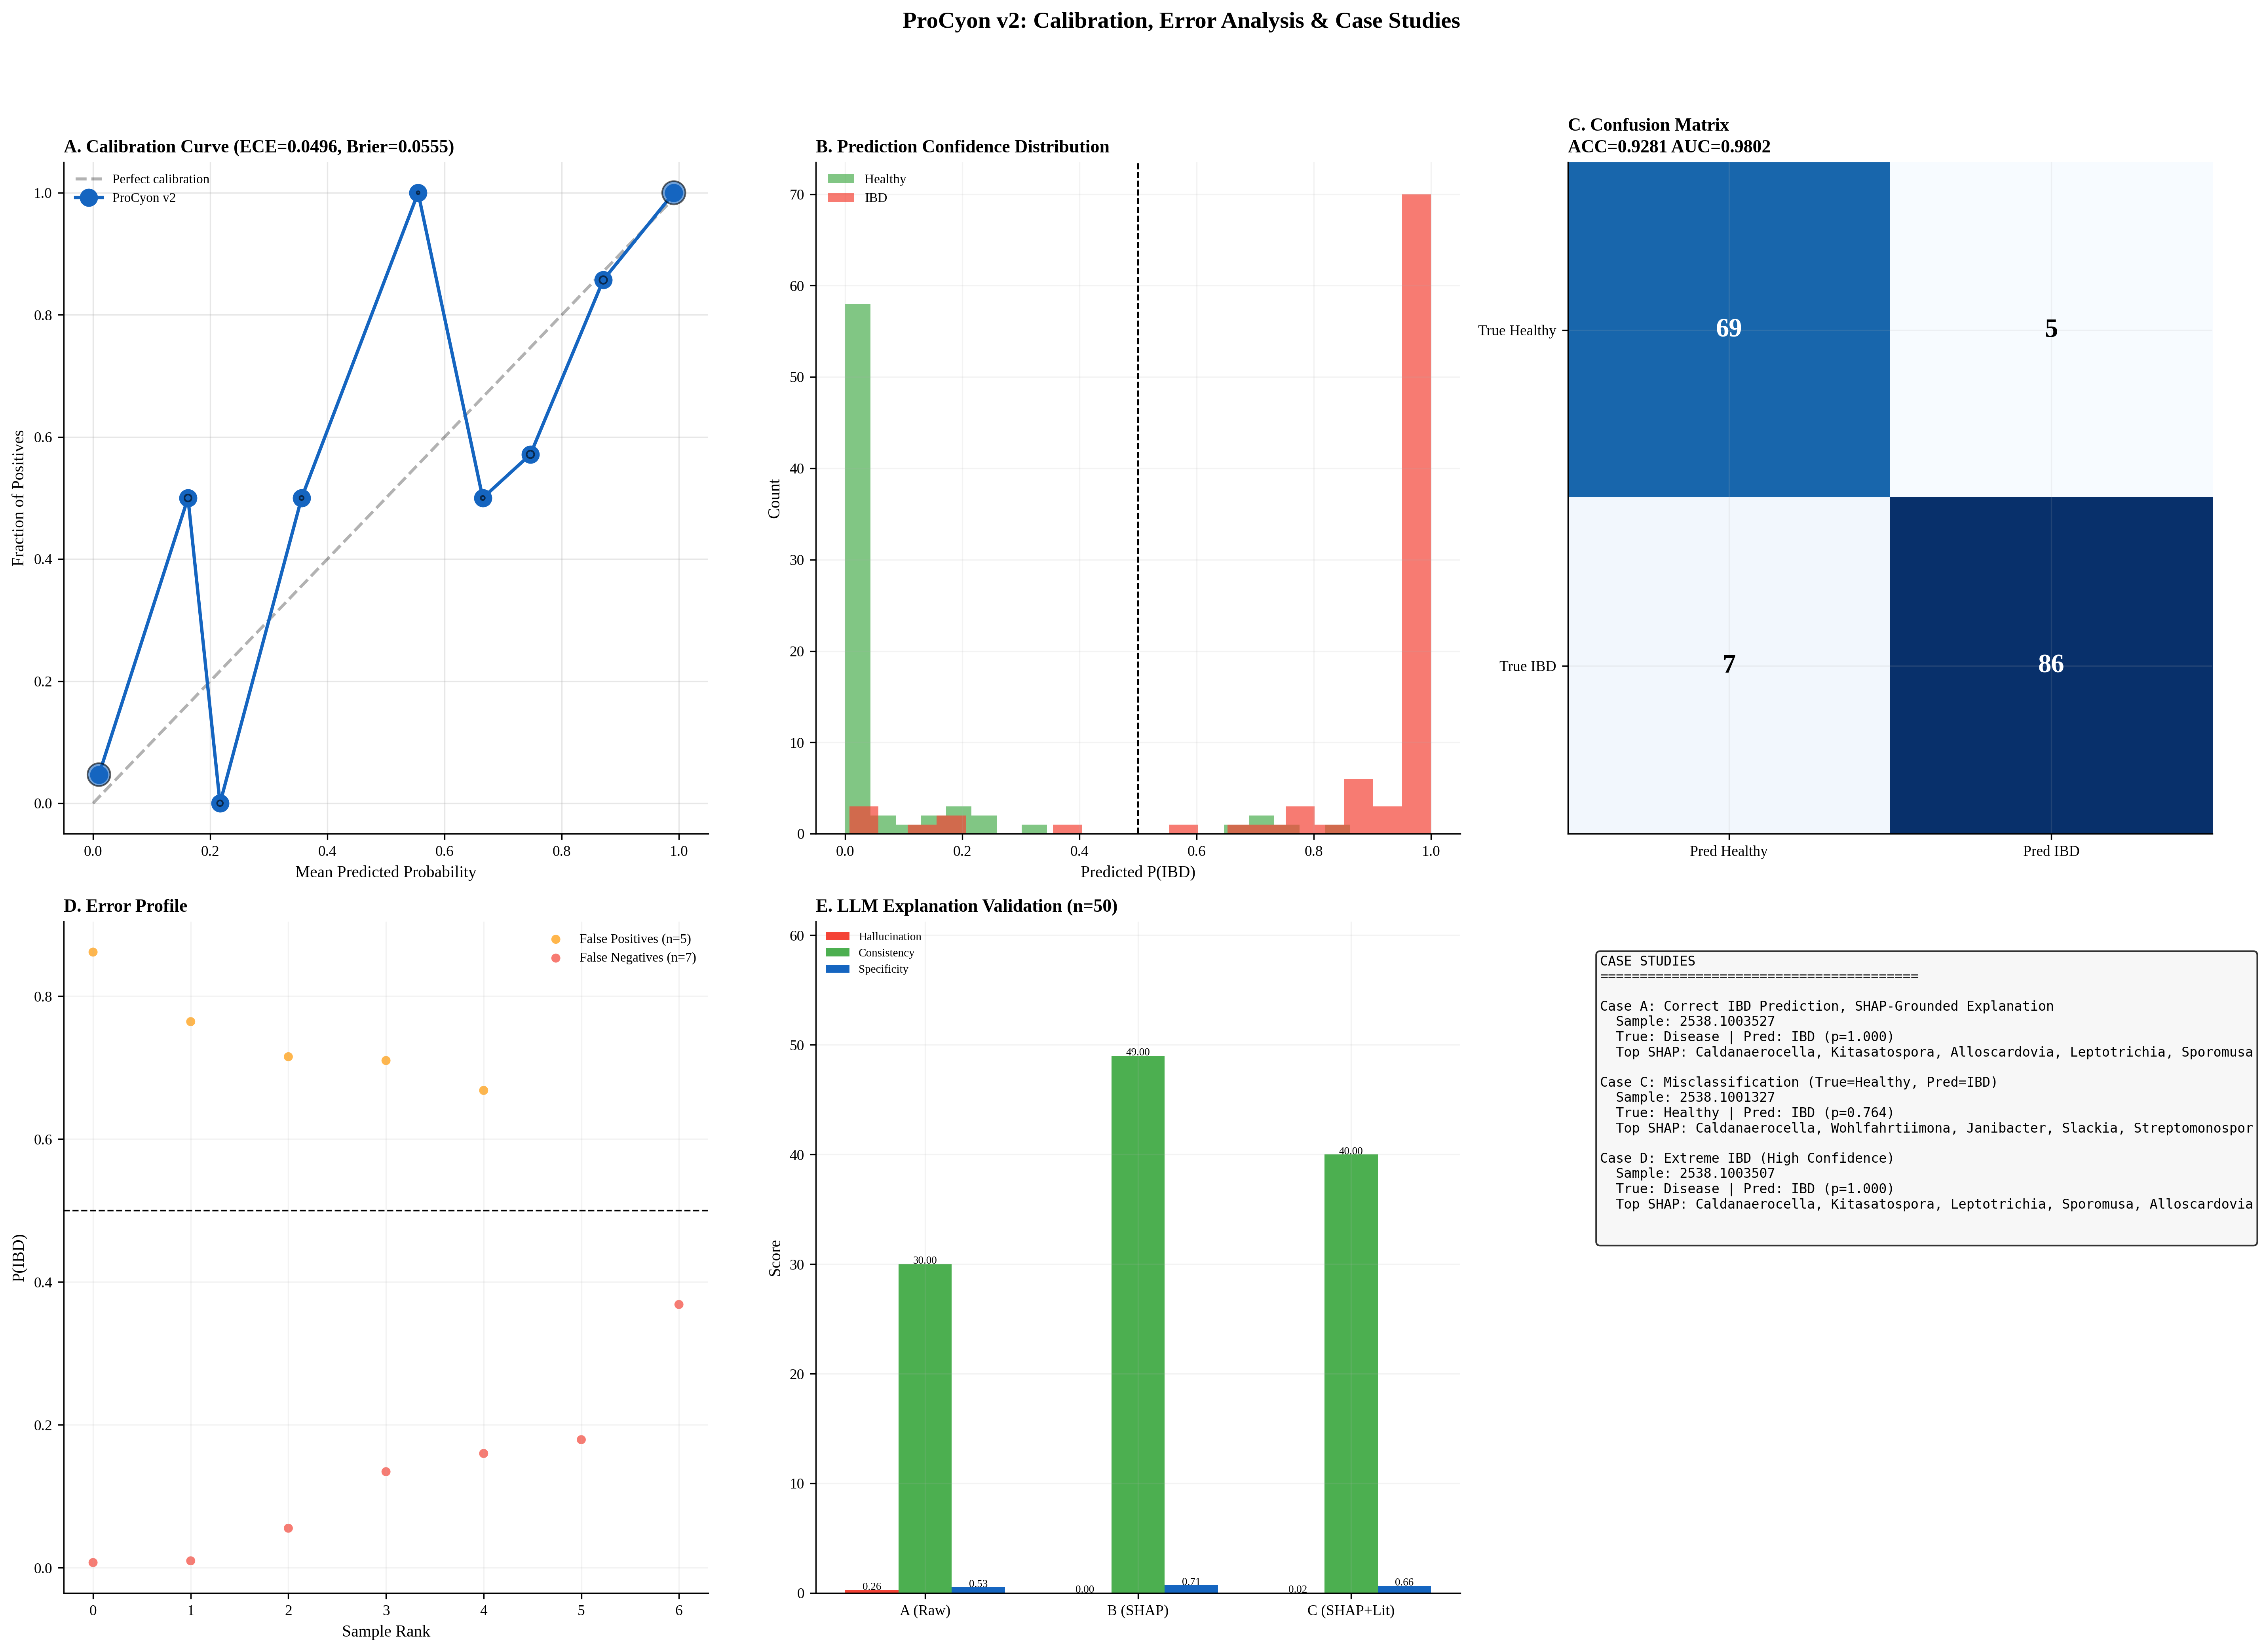
\includegraphics[width=0.95\textwidth]{figures/calibration_error_cases.png}
\caption{\textbf{Calibration, error analysis, and case studies.}
(A) Calibration curve (ECE$=$0.05, Brier$=$0.056). (B) Prediction confidence distribution.
(C) Confusion matrix. (D) Error profile: false positives vs.\ false negatives.
(E) LLM explanation validation summary. (F) Case study overview.}
\label{fig:calibration}
\end{figure}
\begin{figure}[ht]
\centering
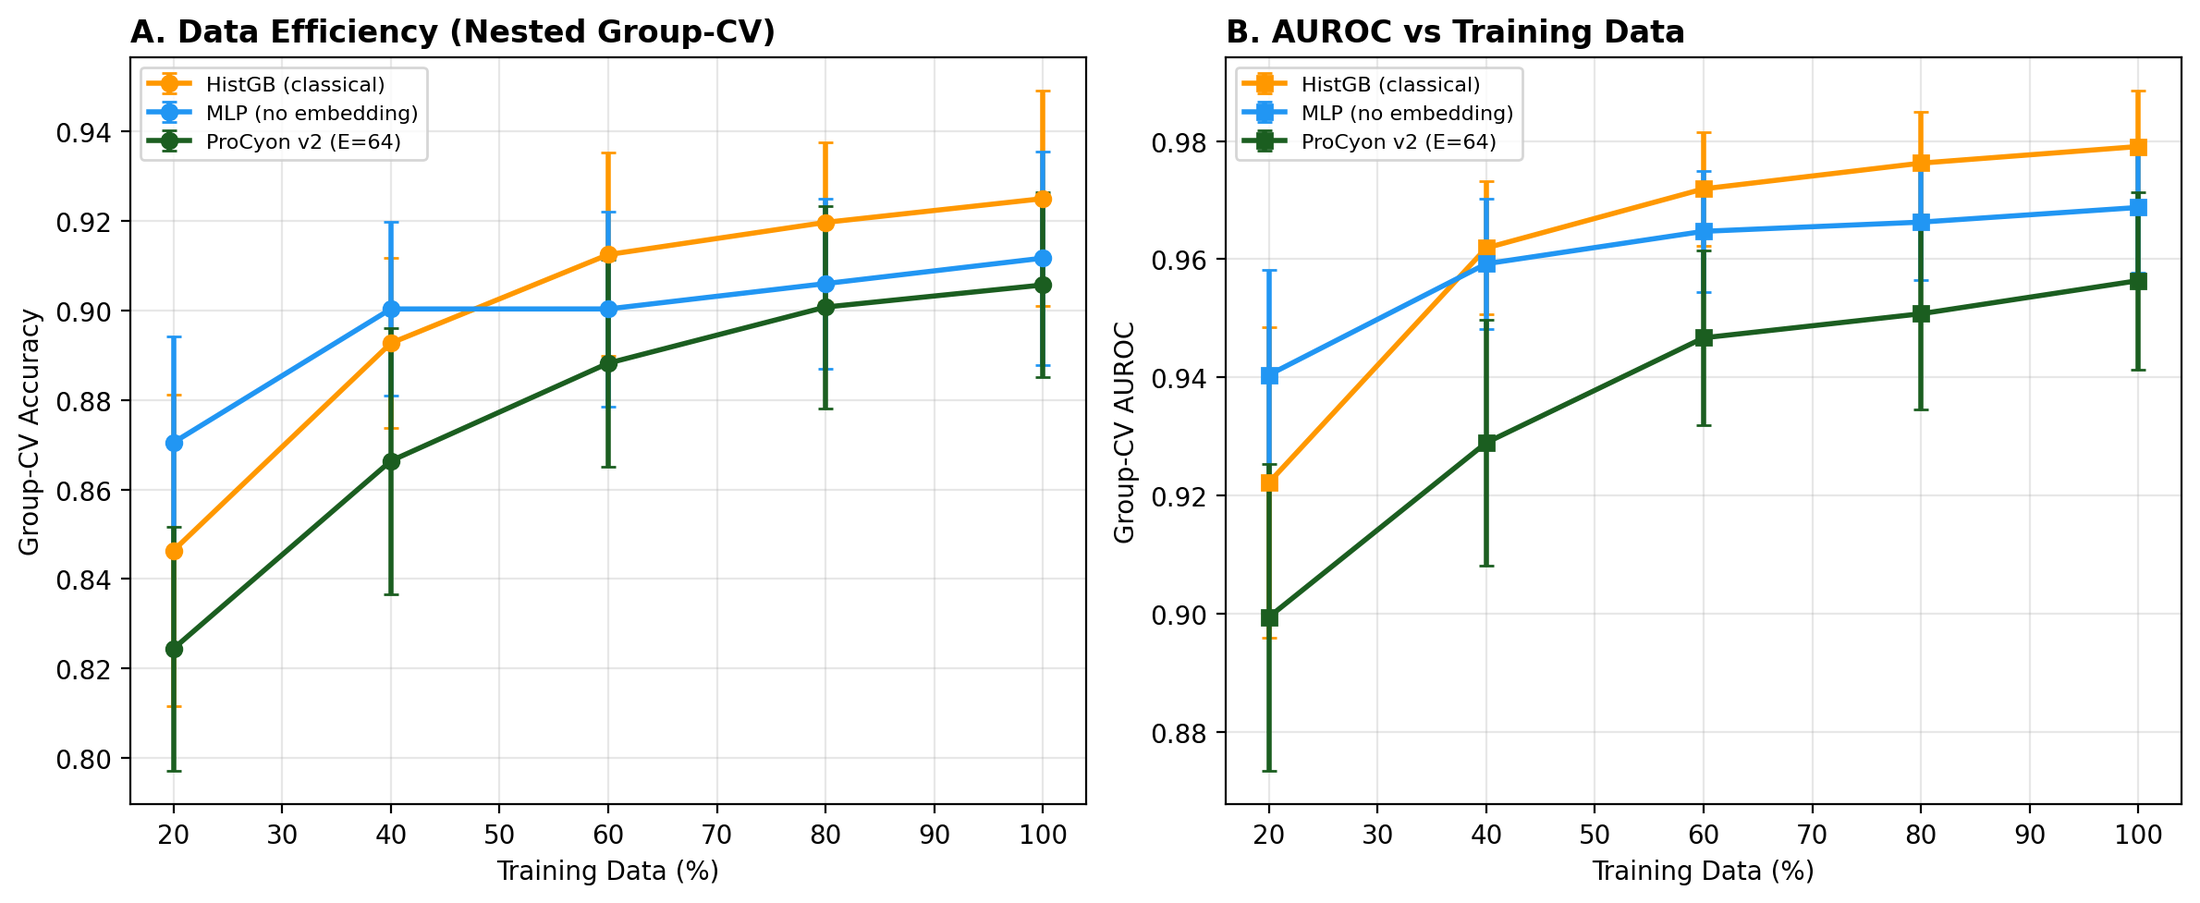
\includegraphics[width=0.85\textwidth]{figures/learning_curve.png}
\caption{\textbf{Data efficiency (nested group-CV).}
(A) Accuracy and (B) AUROC as a function of training data fraction for
HistGradientBoosting, MLP without embedding, and SimpleEmb (E$=$64).}
\label{fig:learning}
\end{figure}

\begin{table}[ht]
\centering
\caption{\textbf{LLM explanation validation (all 167 test samples, Qwen2-7B-Instruct).}
Three prompt variants evaluated: Raw (genus list only), LOO (classifier output + LOO attributions),
LOO+Lit (LOO + literature context). Bold indicates best.}
\label{tab:llm}
\begin{tabular}{p{6.0cm}ccc}
\toprule
\textbf{Metric} & \textbf{Raw LLM} & \textbf{LOO+LLM} & \textbf{LOO+Lit+LLM} \\
\midrule
Hallucinated genera (avg/response) & 0.72 & \textbf{0.36} & 0.35 \\
Input genera mentioned (avg) & 5.47 & 9.02 & \textbf{9.05} \\
LOO consistency (mentioned genera in top-15) & 0.70 & 0.99 & \textbf{1.00} \\
Direction accuracy & 0.27 & \textbf{0.94} & 0.93 \\
Prediction consistency (\%) & 63\% & \textbf{98\%} & 98\% \\
Specificity ratio (biol. mechanisms) & 0.38 & \textbf{0.44} & 0.33 \\
\bottomrule
\end{tabular}
\end{table}
\end{document}
